\phantomsection
\addcontentsline{toc}{chapter}{Timing study of hadronic showers in the AHCAL technological prototype}
\chapter*{Timing study of hadronic showers in the AHCAL technological prototype}
\label{chap:TimingAHCAL}

The International Large Detector (ILD), as described in \ref{}, considers a highly granular hadronic calorimeter using iron absorbers to achieve a compact detector with the best jet energy resolution of around 3-4\% at 250 GeV satisfying the space constrain imposed by the solenoid magnet. Timing measurements in a calorimeter can be used to reject pile-up events, for example at the LHC or CLIC coming from out-of-time pile-up events due to the bunch-to-bunch spacing of 25 (0.5 ns) respectively. The high level of $\gamma\gamma \rightarrow$ hadrons events at CLIC could be rejected by using the timing information from the calorimeter in order to limit the impact of the background on physics measurements. Time information could be used also for improving energy reconstruction \cite{Benaglia2016}.\\

In the hadronic calorimeter, the timing is highly influenced by the time structure of the shower itself. A hadronic shower possesses several timing components depending on the different processes happening in the shower. A fast component related to instantaneous high energy depositions from relativistic hadrons and electromagnetic sub-showers. A slow component due to neutron scattering, nuclear-recoil and photons from nuclear processes. This component can live up to several milliseconds. Apart from physics processes, the measured hit time is influenced by the active medium used as well as by the electronics. Time constants in the active medium, such as scintillation decay time, can affect the measurement.\\

The performance of the ILD relies on simulation studies based on \geant, it is important to study how well the simulation performs to reproduce the time structure of hadronic showers observed in data. The CALICE Analog Hadronic Calorimeter (AHCAL) technological prototype was installed at the SPS CERN facilities in July and August 2015, in order to provide measurements using plastic scintillators. The goal of this study is to improve our knowledge about hadronic showers, especially in terms of its time evolution and the time correlations between layers within the calorimeter. The strategy of this analysis is fairly simple and divided in three parts:
\begin{itemize}
	\item Determination of the time calibration constants using muon data
	\item Cross-check of the time calibration with electron data
	\item Analysis of the pion data
\end{itemize}
This chapter will firstly describe the timing calibration procedure of the AHCAL, followed by the comparison between data and simulation for muons and electrons and finally a comparison with pion data.

\chapter{Runs \& Event Selection}
\label{sec:EvtSelection}

A description of the beanline is available in section \ref{sec:beamline} as well a description of the detector setup in section \ref{sec:TBsetup}.

\section{Trigger Signals}
\label{subsec:trigger}

For a muon beam, two scintillator plates of $50\times50$ cm$^2$ were placed in front of and behind the calorimeter. For electron and pion beams, two small scintillator plates of $10\times10$ cm$^2$ were positioned in front of the calorimeter. The trigger scintillators were connected to a NIM-logic (discriminator and gate) in order to provide a validation signal to the SPIROC readout ASIC (see section \ref{}).
In order to provide the signal of the trigger scintillators to be used as a time reference, a SiPM-like pulse of around 4 $\mu$s length and with a fast rising edge of around 1 ns was generated from the NIM-logic with an amplitude around 100 mV. This signal was injected directly via AC coupling to some electronics channels in the setup as shown in table \ref{table:trigger_signal_list}. No other external time reference than these channels was available. In the following analysis, only the reference signals T$_{12}$,  T$_{13}$ and T$_{14}$ were used. The channels were determined to be noisy or broken by looking at the energy spectra of theses channels. Broken channels resulted in an empty energy spectra and noisy channels were showing two energy peaks, one near pedestal and another at the expected energy value.

\begin{table}[htb!]
	\centering
	\caption{List of channels with the injected trigger signal to be used as time reference.}
	\label{table:trigger_signal_list}
	\begin{tabular}{@{} ccccc @{}}
		\hline
		Layer \# & Chip Number & Channel & Comments & Name \\
		\hline
		11 & 169 & 29 & noisy & T$_{11}$ \\
		11 & 177 & 23 & broken & - \\
		12 & 185 & 29 & - & T$_{12}$ \\
		13 & 201 & 29 & -  & T$_{13}$ \\
		13 & 211 & 6 & broken & - \\
		14 & 217 & 23 & - & T$_{14}$ \\
		\hline
	\end{tabular}
\end{table}

\section{Dataset}
\label{subsec:dataset}

During the campaign at SPS in July 2015, $\mu^-$ runs were taken at 50 and 150 GeV beam energy for the calibration of the detector. Several e$^{-}$ runs were taken between 10 to 50 GeV beam energy to study the electromagnetic response of the calorimeter. The e$^{-}$ runs were quite pure as the beam was generated via a neutral beam directed on a converter target. %Due to the significant amount of air and beam line instrumentation between the calorimeter and the final momentum selection magnet as well as few information of the beam parameters, the beam profile of electron runs is not well reproduced in simulation.%
Finally, $\pi^-$ runs were taken between 10 to 90 GeV beam energy. The table \ref{table:dataruns} sums up the dataset taken. The number of events that are shown in the table are the total number of collected events.

\begin{table}[htb!]
	\centering
	\caption{List of runs taken at SPS in July 2015.}
	\label{table:dataruns}
	\resizebox{0.9\textwidth}{!}{%
	\begin{tabular}{@{}l||p{2cm}p{7.5cm}p{2cm}@{}}
		\hline
		\multicolumn{1}{l}{\textbf{Particle}} & \textbf{Energy} & \textbf{Runs} & \textbf{\# Events}\\
		\hline
		\multirow{2}{*}{$\mu^-$}& 50 GeV & 24016-24204 & 120,887,651\\& 150 GeV & 24623-24662 & 15,534,328\\
		\hline
		\multirow{2}{*}{e$^-$}& 10 GeV & 24531-24576 & 38,028,438\\& 15 GeV & 24507-24527 & 7,701,325\\& 20 GeV & 24479-24504 & 10,498,554\\& 30 GeV & 24454-24475 & 3,382,943\\& 40 GeV & 24420-24448 & 2,665,843\\& 50 GeV & 24404-24419 & 5,933,995\\
		\hline
		\multirow{2}{*}{$\pi^-$}& 10 GeV & 24266-24272, 24300-24317, 24381-24397 & 24,311,420\\& 20 GeV & 24398-24400 & N/A\\& 30 GeV & 24259-24299, 24319-24380 & 10,120,753\\& 50 GeV & 24212-24254, 24325-24357, 24580-24612 & 10,704,661\\& 70 GeV & 24219-24242, 24365-24374 & 8,885,407\\& 90 GeV & 24233-24287, 24331-24364 & 7,955,604\\
		\hline
	\end{tabular}
	}
\end{table}

\section{MIP Pre-selection}
\label{subsec:Muon_presel}

A clean selection of MIP tracks is needed in order to obtain and cross-check the MIP calibration at a single cell level. A simple pre-selection was performed on the muon sample designed to select effectively MIP-like particles going through the AHCAL. In a second step, a track selection was performed to retain only MIP-like particle as explained in subsection \ref{subsec:Muon_sel}.

The pre-selection is based on the center of gravity $cog_Z$ and the number of hits $n_{Hits}$. A MIP-like particle should, in principle, deposit the same energy in each layer of the calorimeter thus the center of gravity should be roughly centered in the calorimeter in the z coordinate. As well, the number of hits should be around 1 per layer for a MIP-like particle plus accounting for some possible noise in the detector thus explaining the cut at $n_{Hits} = 20$.

The AHCAL distribution of $cog_Z$ vs $n_{Hits}$ obtained from simulated 50 GeV muons, electrons and pions and the applied pre-selection is shown in figure \ref{fig:Muons_CoGZ_nHits}. The pre-selection efficiency is 99.4\% for muons, 0\% for electrons and 13.3\% for pions.

\begin{figure}[htbp!]
	\centering
	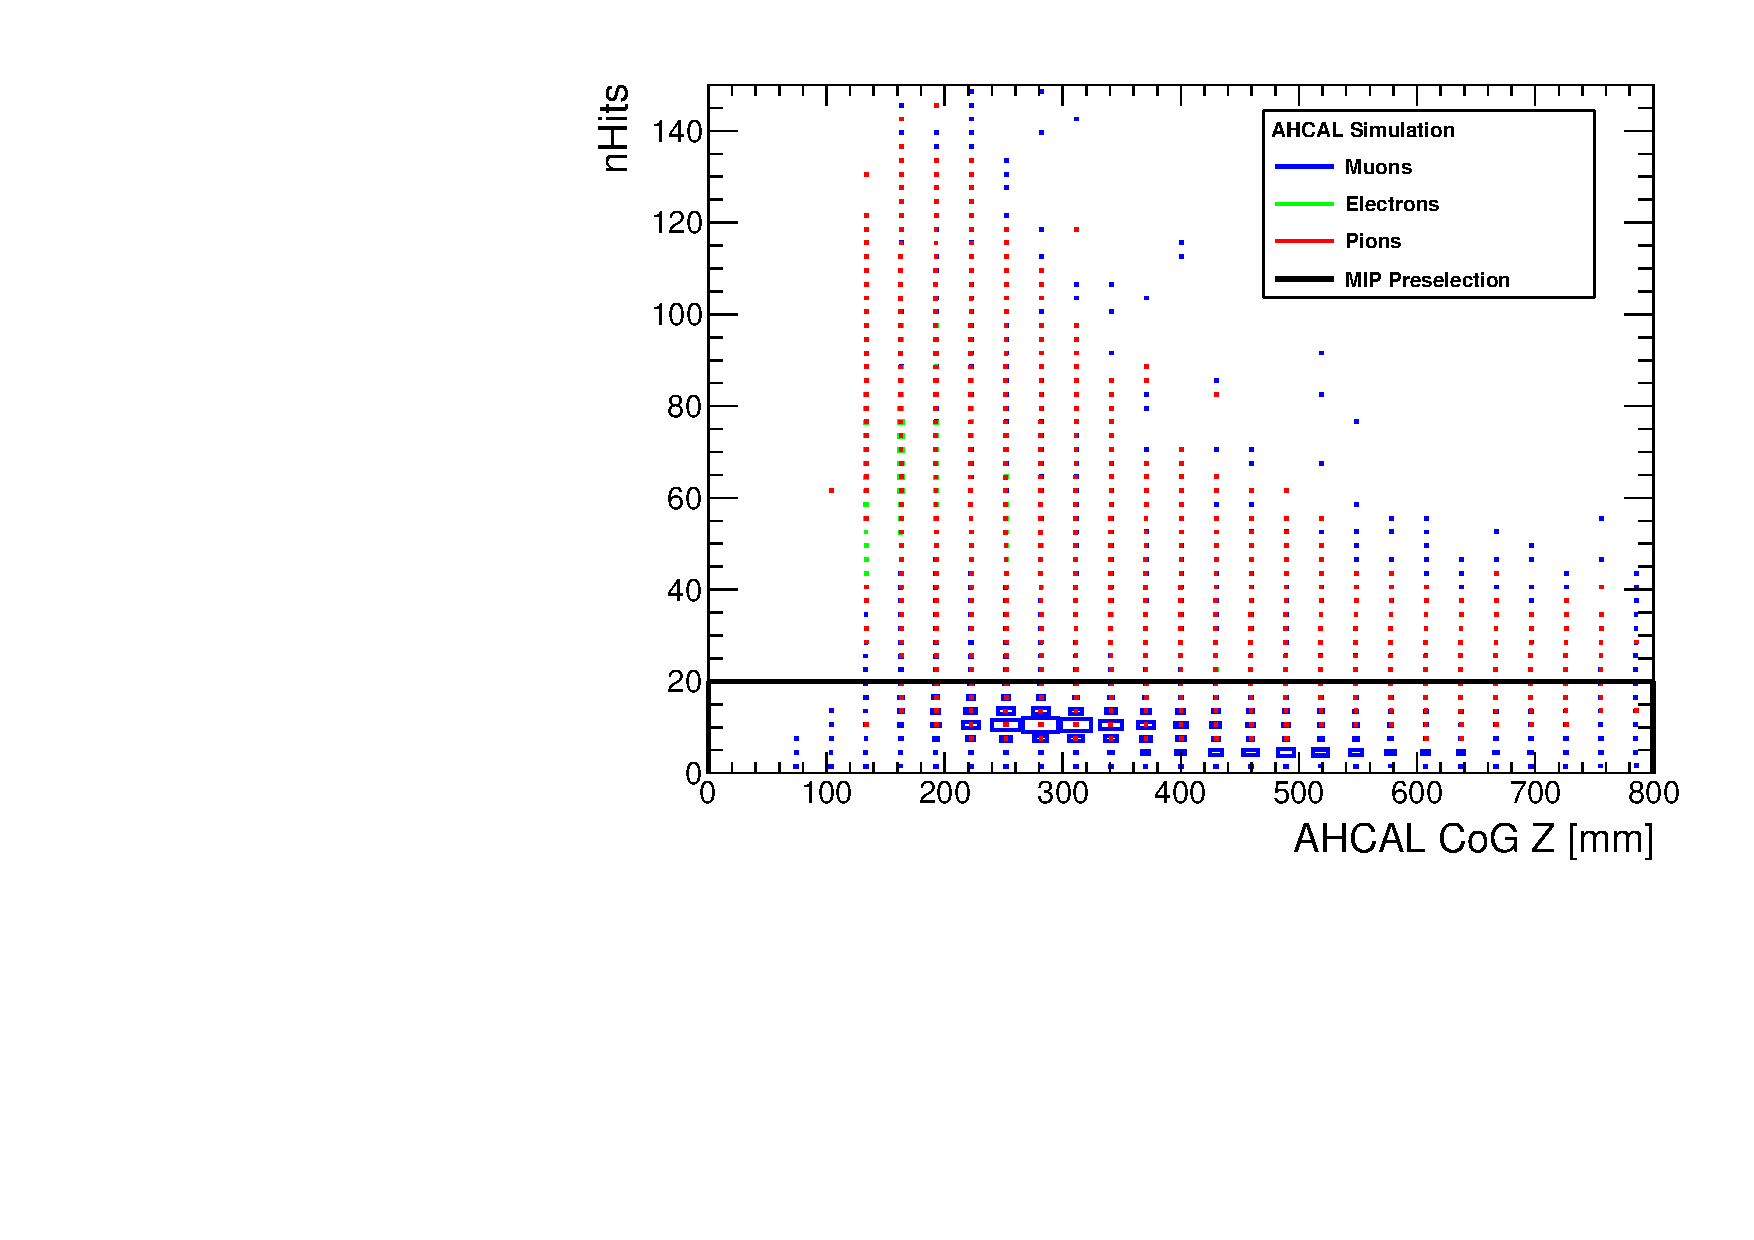
\includegraphics[width=0.7\linewidth]{../Thesis_Plots/Timing/Muons/Plots/SelectionCut_nHitsCoGZ_Muons}
	\caption{Event distribution in $cog_Z:n_{Hits}$ plane. The black box represents the space-phase covered by the pre-selection.} \label{fig:Muons_CoGZ_nHits}
\end{figure}

\section{MIP Selection}
\label{subsec:Muon_sel}

The muon runs were taken first at 50 GeV then another scan at the end of the campaign was performed at 150 GeV. The muon beam was produced by scraping the halo of a secondary pion beam using collimators. After investigation, muon runs were contaminated by pions. A simple estimation by looking at the spectrum of the number of hits per event provided that around 30\% of the events were contaminated by pions.

The muon selection was designed to efficiently select muons and reject late pion showers. For this, a simple MIP track-finder has been developed based on pre-existing work \cite{Hartbrich:2016bbz}. The algorithm selects AHCAL towers of hits in the same $x:y$ position and rejects towers under a certain number of hits. In order to select muons or punch through pions, a straight track of at least 7 hits is required in the whole AHCAL without a hard interaction. This also assumes that the calorimeter was perfectly perpendicular to the beam, any tilted tracks would be missed. In addition to reject late pion showers, no more than 2 hits are allowed per layer accounting for some flexibility with noise hits. The distributions of the maximum number of hits in a layer and the number of hits of a track are shown in figures \ref{fig:Muons_Track_nHitsLayer} and \ref{fig:Muons_Track_nHits} for simulated samples of 50 GeV muons, electrons and pions after pre-selection. The track-finder was performed in two steps for the inner part of the detector of $12 \times 12$ tiles and the outer part of the big layers (BL) in order to catch the halo of muons.

The selection efficiency is 72.5\% for muons, 0\% for electrons and 5.6\% for pions. The selection reduces further the pion contamination and the remaining pion fraction is compatible with the fraction of pions traversing the AHCAL without hard interaction by calculation. A detailed overview of the MIP selection is given in table \ref{table:muon_sel}.

\begin{figure}[htbp!]
	\begin{subfigure}[t]{0.5\textwidth}
		\centering
		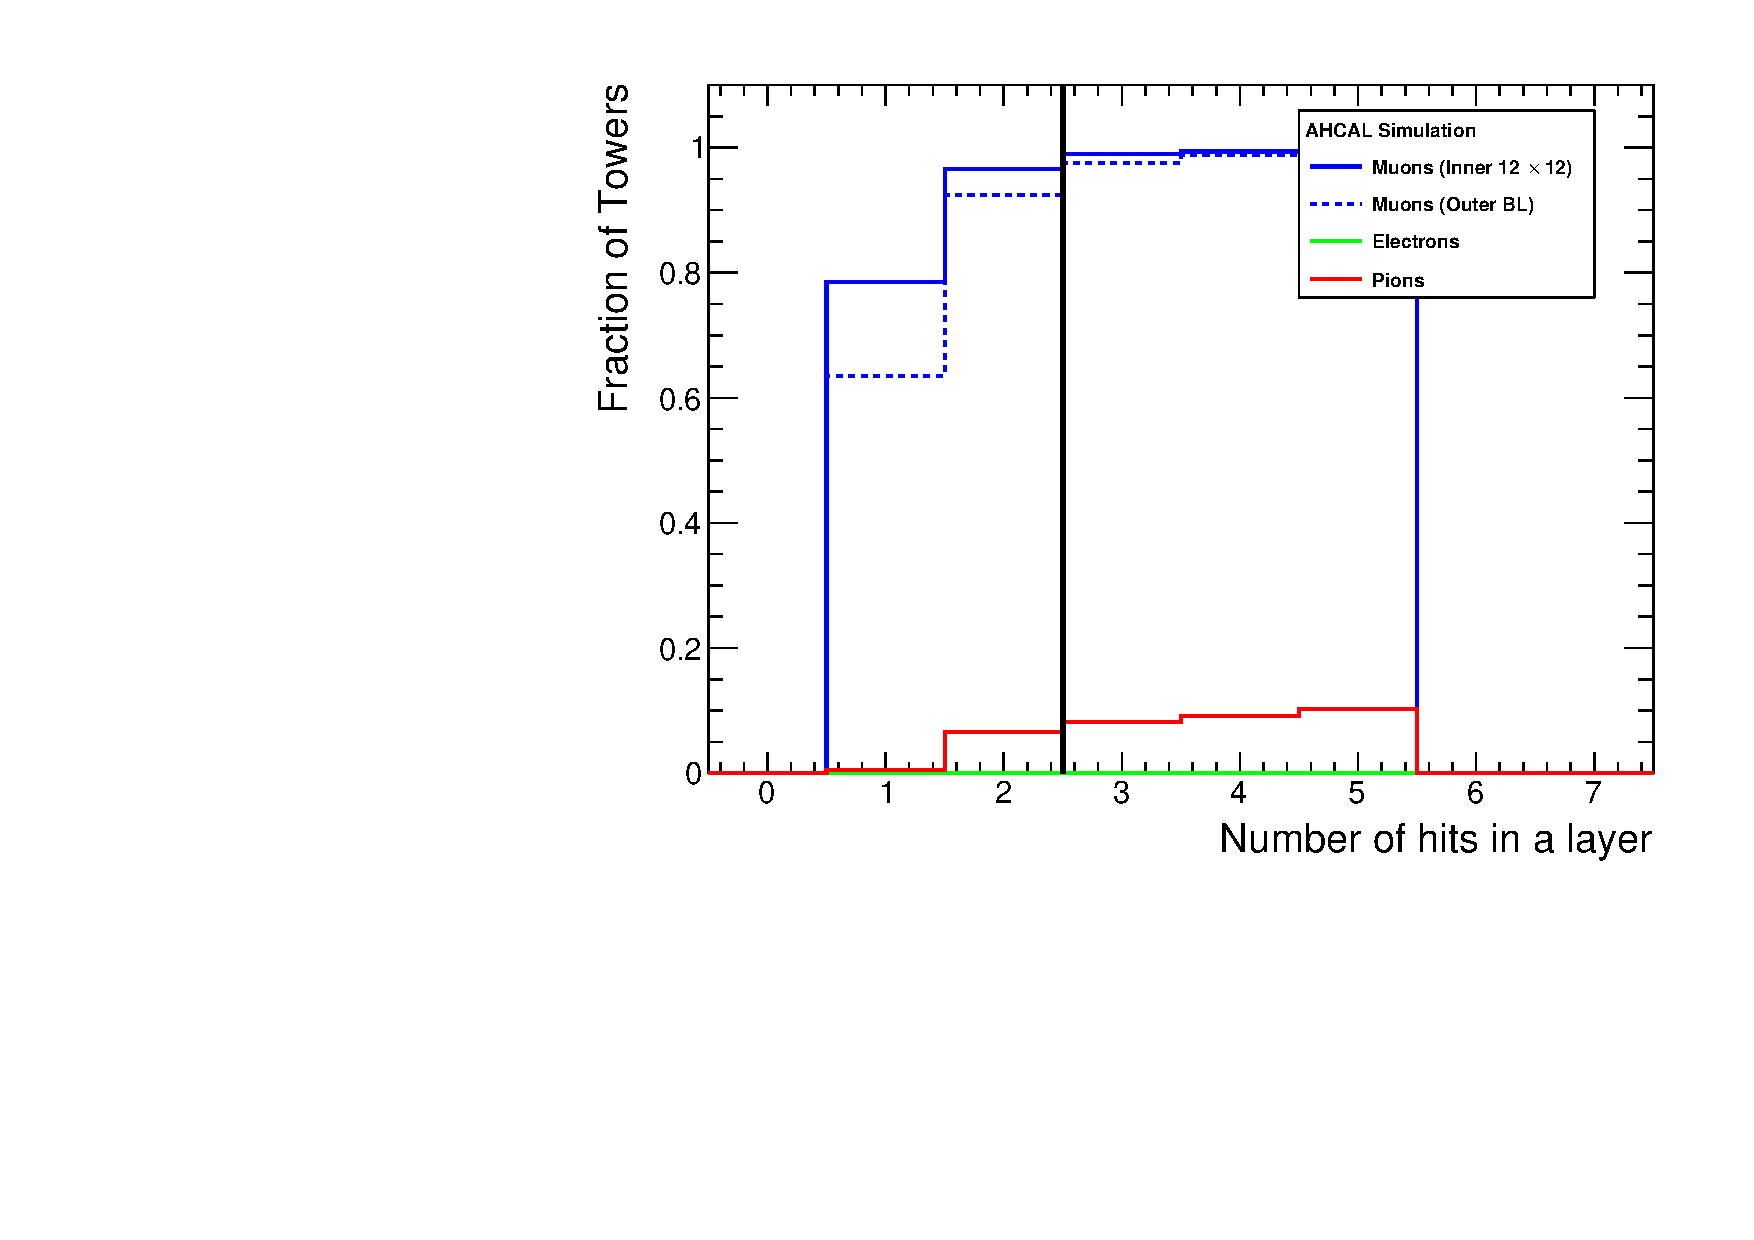
\includegraphics[width=1\linewidth]{../Thesis_Plots/Timing/Muons/Plots/TrackFinderCut_nHitsLayer_Muons}
		\caption{Number of hits in a layer normalized to the number of events.} \label{fig:Muons_Track_nHitsLayer}
	\end{subfigure}
	\hfill
	\begin{subfigure}[t]{0.5\textwidth}
		\centering
		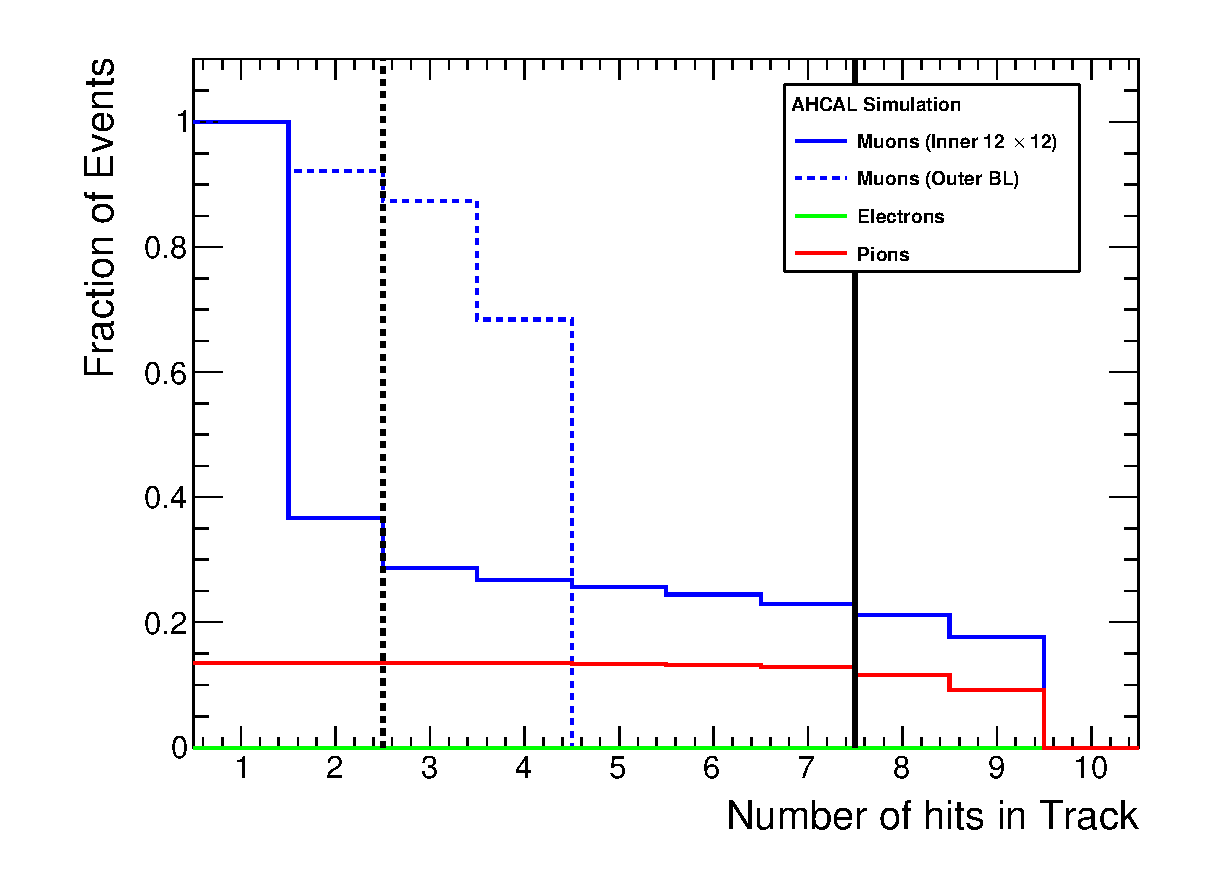
\includegraphics[width=1\linewidth]{../Thesis_Plots/Timing/Muons/Plots/TrackFinderCut_nHitsTrack_Muons}
		\caption{Number of hits in a track normalized to the number of events.} \label{fig:Muons_Track_nHits}
	\end{subfigure}
	\caption{\subref{fig:Muons_Track_nHitsLayer}) Distribution of number of hits in a layer for simulated muons, electrons and pions at 50 GeV. The black line represents the cut of the maximum allowed number of hits in a layer applied for the MIP selection. \subref{fig:Muons_Track_nHits}) Distribution of the number of hits in a track for simulated muons, electrons and pions at 50 GeV. A Tower size of 7 for the inner detector and 2 for the outer big layers was chosen.}
\end{figure}

\section{Electron Selection}
\label{subsec:elec_sel}

The electron selection is done to simply extract single electron showers contained in the AHCAL. These events are needed in order to validate the timing behavior in simulation as well as the detector simulation model. It is important to have a clean sample of electrons to cross-check the timing calibration. For the selection, an \textit{Event Quality} pre-selection is done using the beam instrumentation and layer information. Only events with a Cherenkov tag (only applied on data) are used and the energy in the three first layers of the AHCAL ($E_3+E_4+E_5$) must be over 10 MIP. Distributions of the energy in the three first layer of the AHCAL for simulated 10 and 50 GeV muons, electrons and pions can be seen in figures \ref{fig:e10GeV_E3} and \ref{fig:e50GeV_E3}.

In a next step, the electron selection is performed. Due to the number of unusable layers especially the front ECAL layers (see section \ref{}) and the fact that the detector is not fully equipped, an alternative selection, in contrary to use a shower start finder, needed to be performed to effectively select electrons. As no look into calorimeter linearity and energy resolution is done in this thesis, a cut on the number of hits per event ($n_{Hits}$) versus the center of gravity in z ($CoG_Z < 250 mm$) can be done. This does not induce any bias for a timing analysis, just would only reduce the event statistics.

To ensure a complete containment of the shower and a rejection of possible pion showers, an additional cut on the energy fraction deposited in the last two layers ($(E_{13}+E_{14})/\Sigma E$) is done and required to be under 1\%. Distributions of each variables used in the selection are shown in figures \ref{fig:electronselection} for simulated 10 GeV and 50 GeV muons, electrons and pions. Due to the restriction on the number of hits per event, the cuts are energy dependent. Additionally to reduce transverse leakage, the shower center of gravity in X and Y needs to be within -90 mm and 90 mm. This cut is wider than the trigger scintillator but has no significant impact.

The selection cuts are summarized in table \ref{table:electron_sel} for each energy. The selection efficiencies for beam energies between 10 and 50 GeV are shown in table \ref{table:eff_electron} obtained from simulated samples of muons, electrons and pions with the QGSP\_BERT\_HP physics list.

\begin{table}[htb!]
	\centering
	\caption{Efficiency of the electron selection for simulated electrons, muons and pions for energies between 10 and 50 GeV.}
	\label{table:eff_electron}
	\begin{tabular}{@{} llll @{}}
		\hline
		\textbf{Beam Energy} & \textbf{$\epsilon_{\mu}$} & \textbf{$\epsilon_{e}$} & \textbf{$\epsilon_{\pi}$}\\
		\hline
		10 GeV & <0.1\% & 96\% & 15.9\%\\
		15 GeV & <0.1\% & 95.7\% & 10.1\%\\
		20 GeV & <0.1\% & 95.2\% & 6.3\%\\
		30 GeV & <0.1\% & 93.9\% & 2.3\%\\
		40 GeV & <0.1\% & 92.7\% & 1.2\%\\
		50 GeV & <0.1\% & 91.5\% & 1.1\%\\
		\hline
	\end{tabular}
\end{table}

One can notice that a significant fraction of pions is present at low beam energies (10 to 20 GeV). But as the production of electrons in the beamline was done using a beam of photons on a beryllium target, it is believe that there is no pion contamination in the data. Thus no additional cut is needed.

\begin{figure}[htbp!]
	\begin{subfigure}[t]{0.5\textwidth}
		\centering
		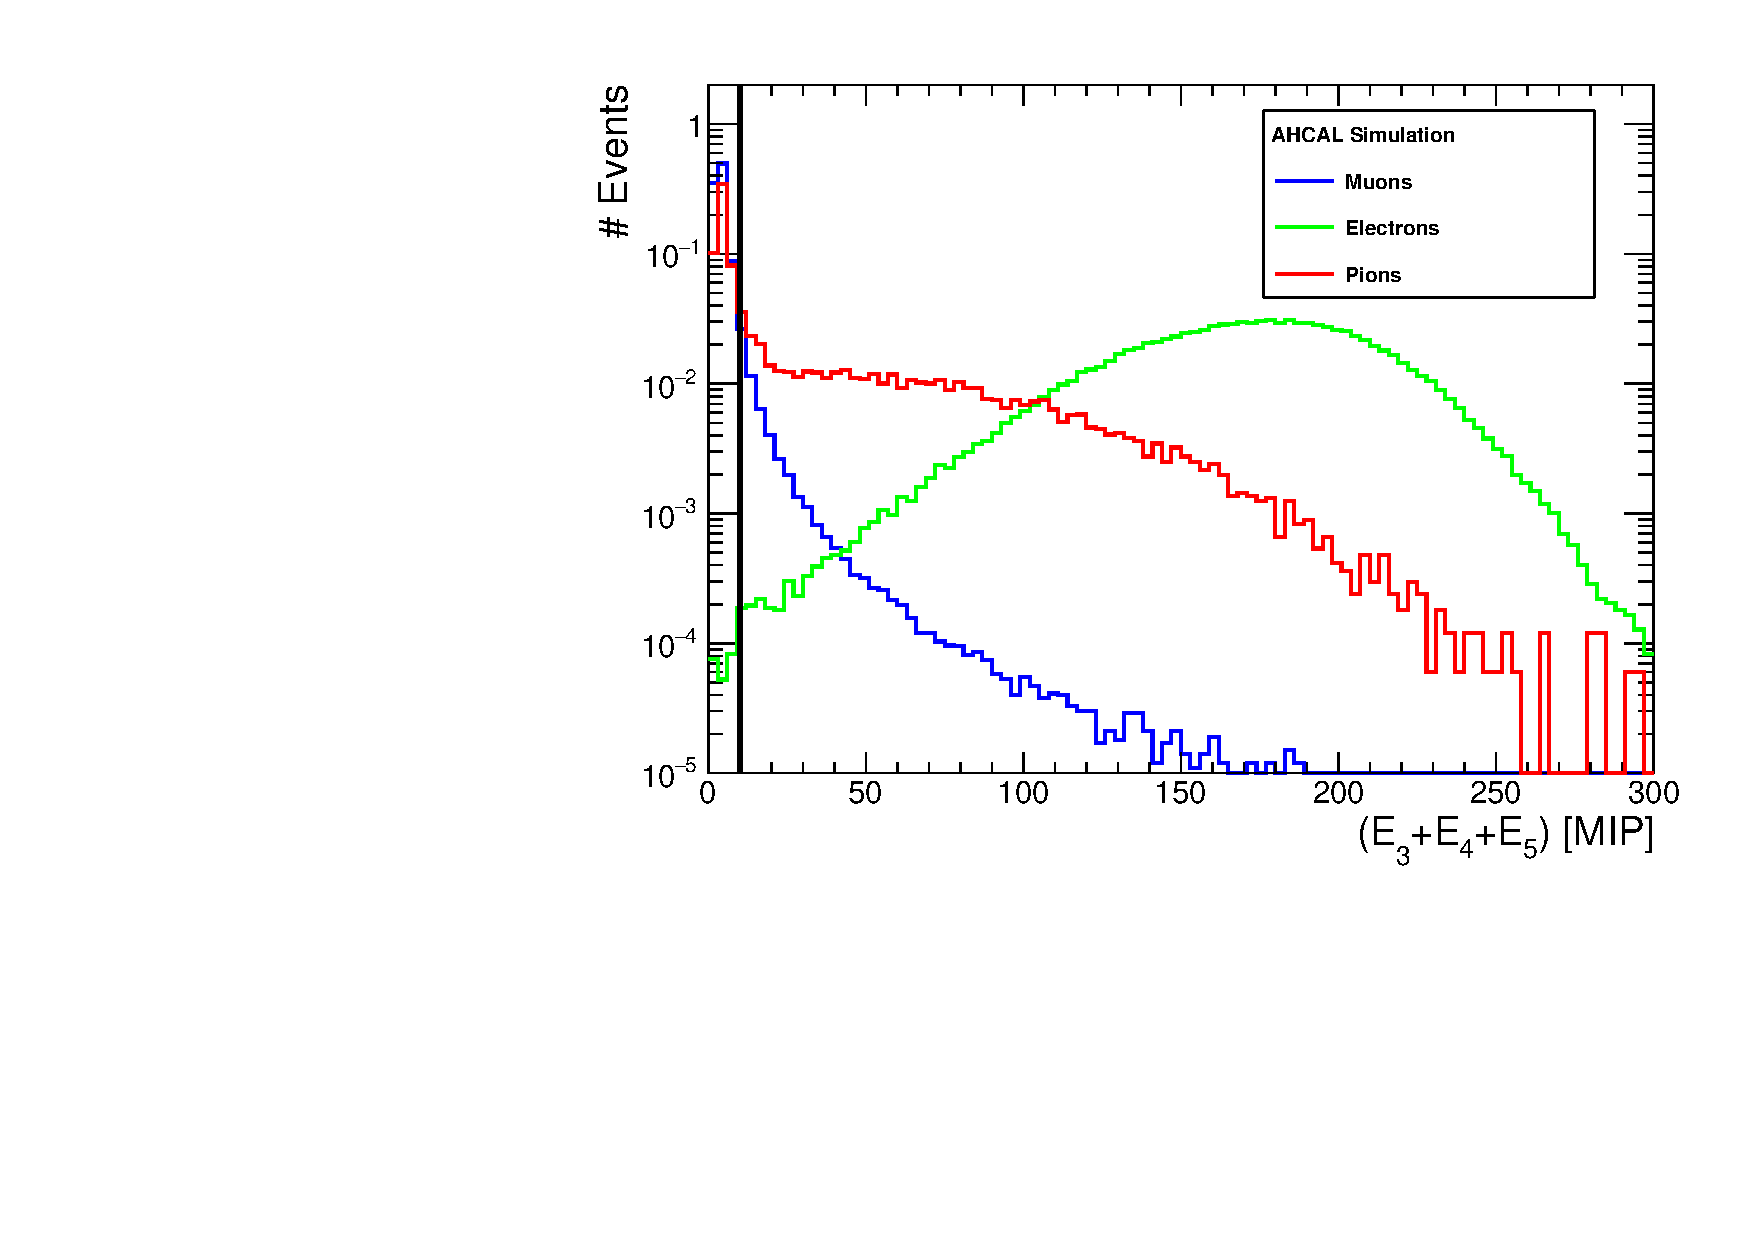
\includegraphics[width=1\linewidth]{../Thesis_Plots/Timing/Electrons/Plots/SelectionCut_EnergyE3_10GeV}
		\caption{10 GeV.} \label{fig:e10GeV_E3}
	\end{subfigure}
	\hfill
	\begin{subfigure}[t]{0.5\textwidth}
		\centering
		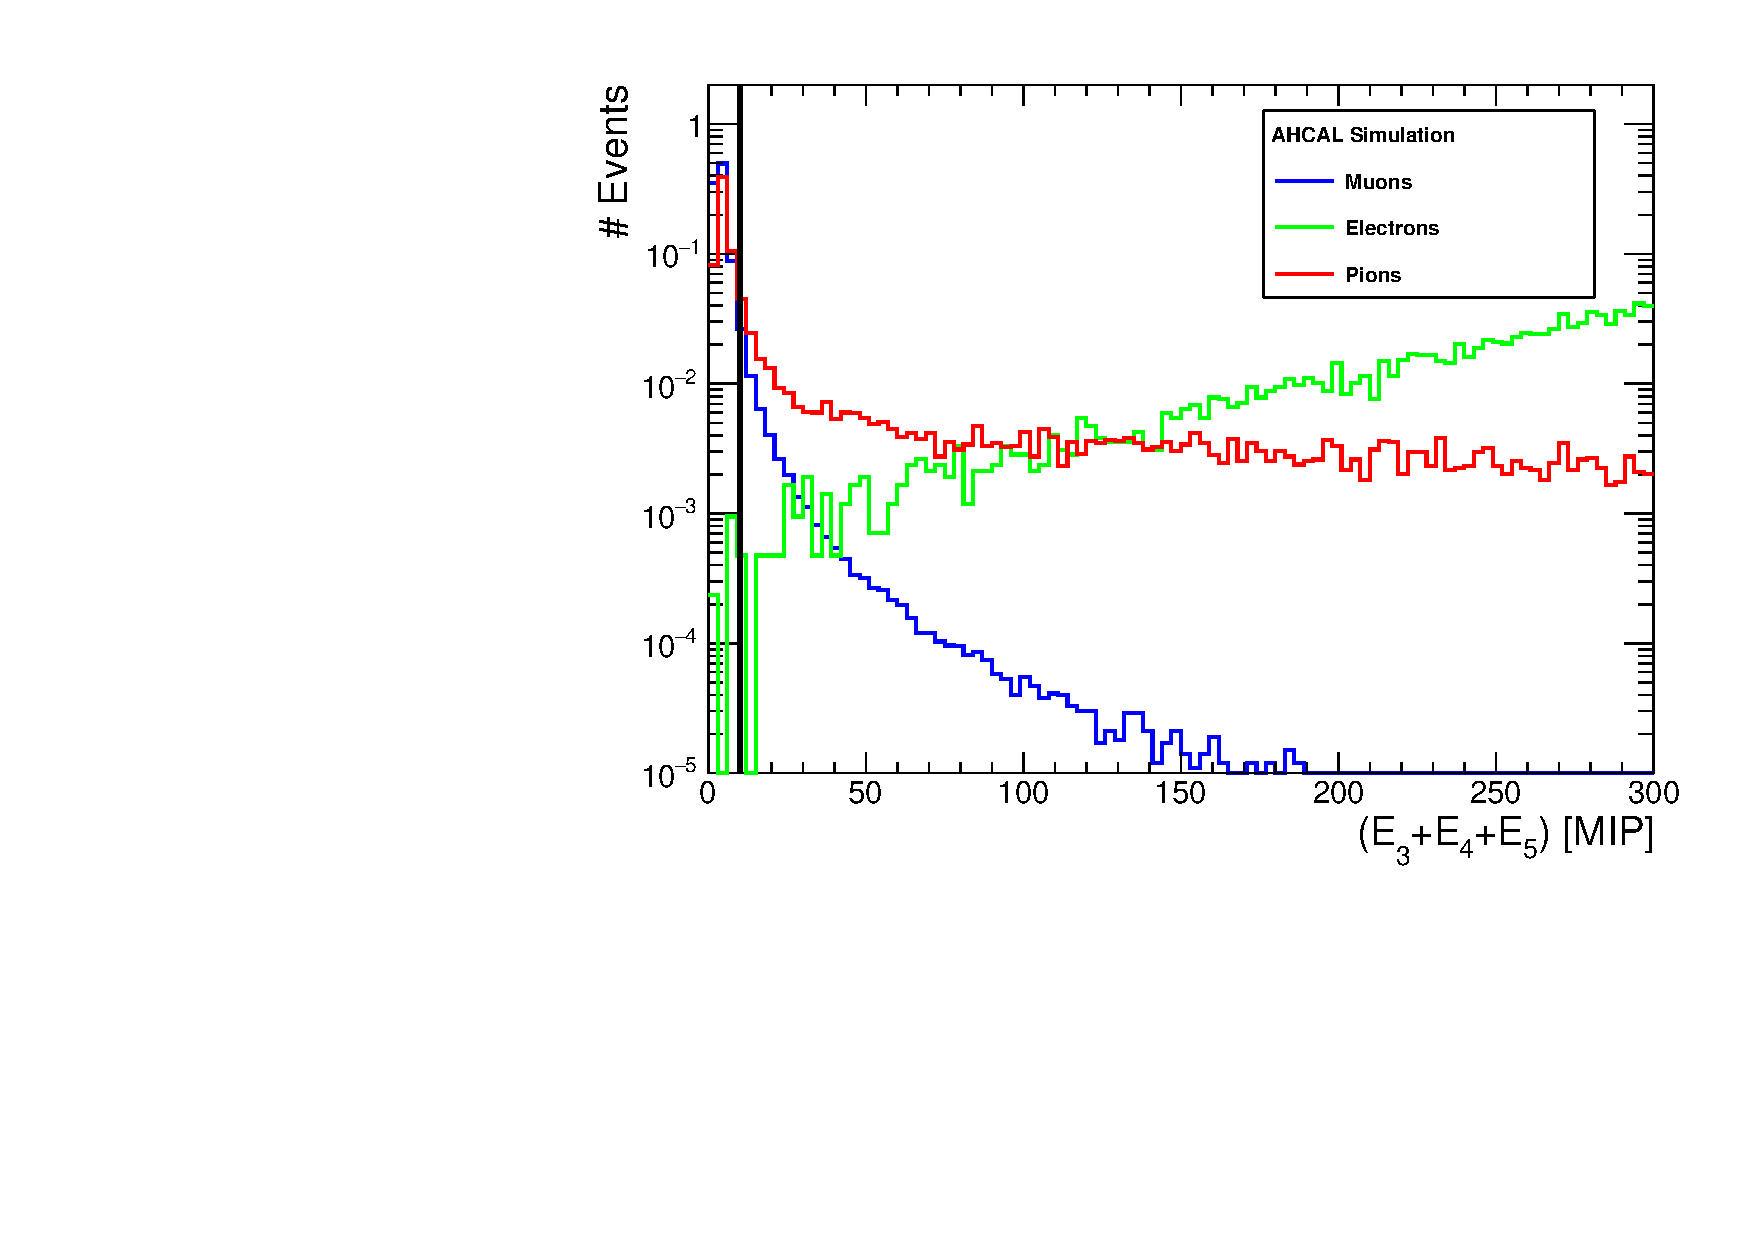
\includegraphics[width=1\linewidth]{../Thesis_Plots/Timing/Electrons/Plots/SelectionCut_EnergyE3_50GeV}
		\caption{50 GeV.} \label{fig:e50GeV_E3}
	\end{subfigure}
	\hfill
	\begin{subfigure}[t]{0.5\textwidth}
		\centering
		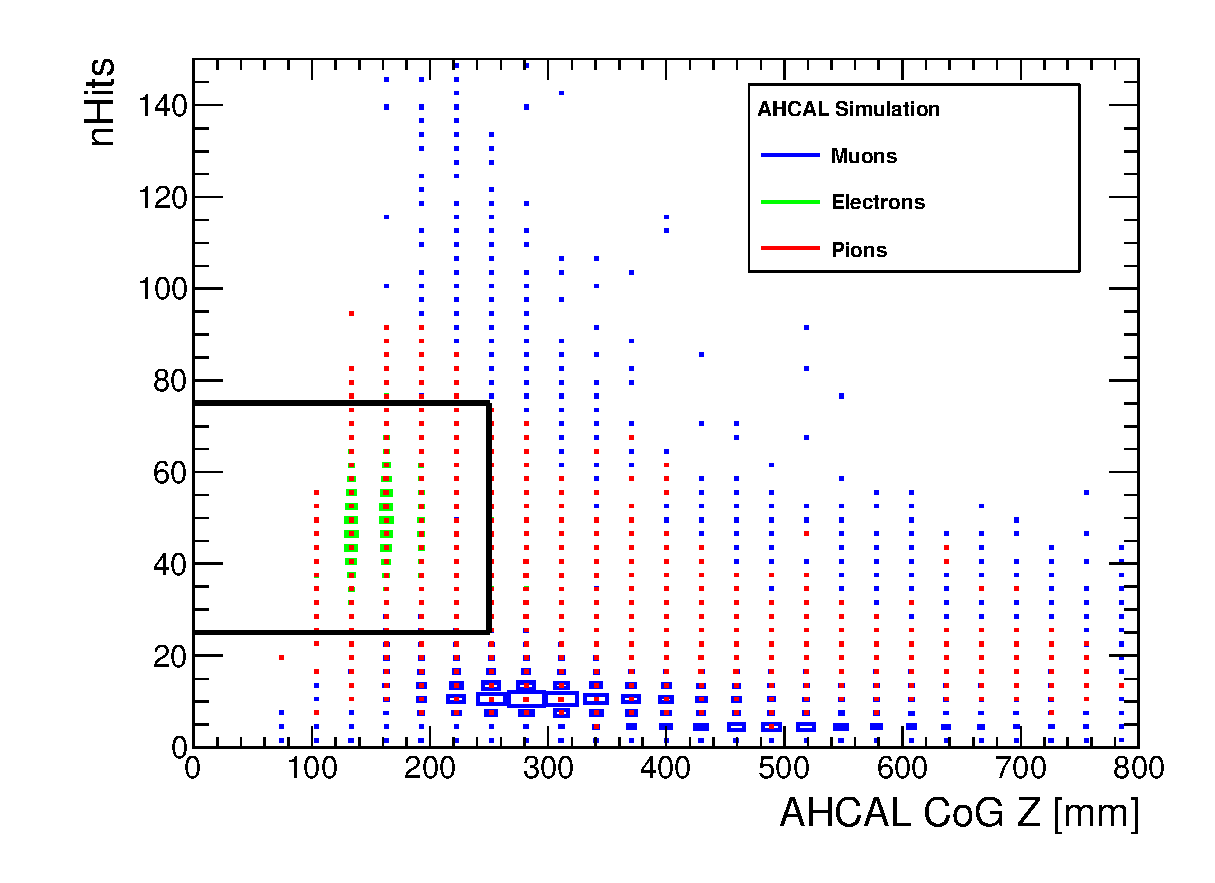
\includegraphics[width=1\linewidth]{../Thesis_Plots/Timing/Electrons/Plots/SelectionCut_nHitsCoGZ_10GeV}
		\caption{10 GeV.} \label{fig:e10GeV_nHitsCoGZ}
	\end{subfigure}
	\hfill
	\begin{subfigure}[t]{0.5\textwidth}
		\centering
		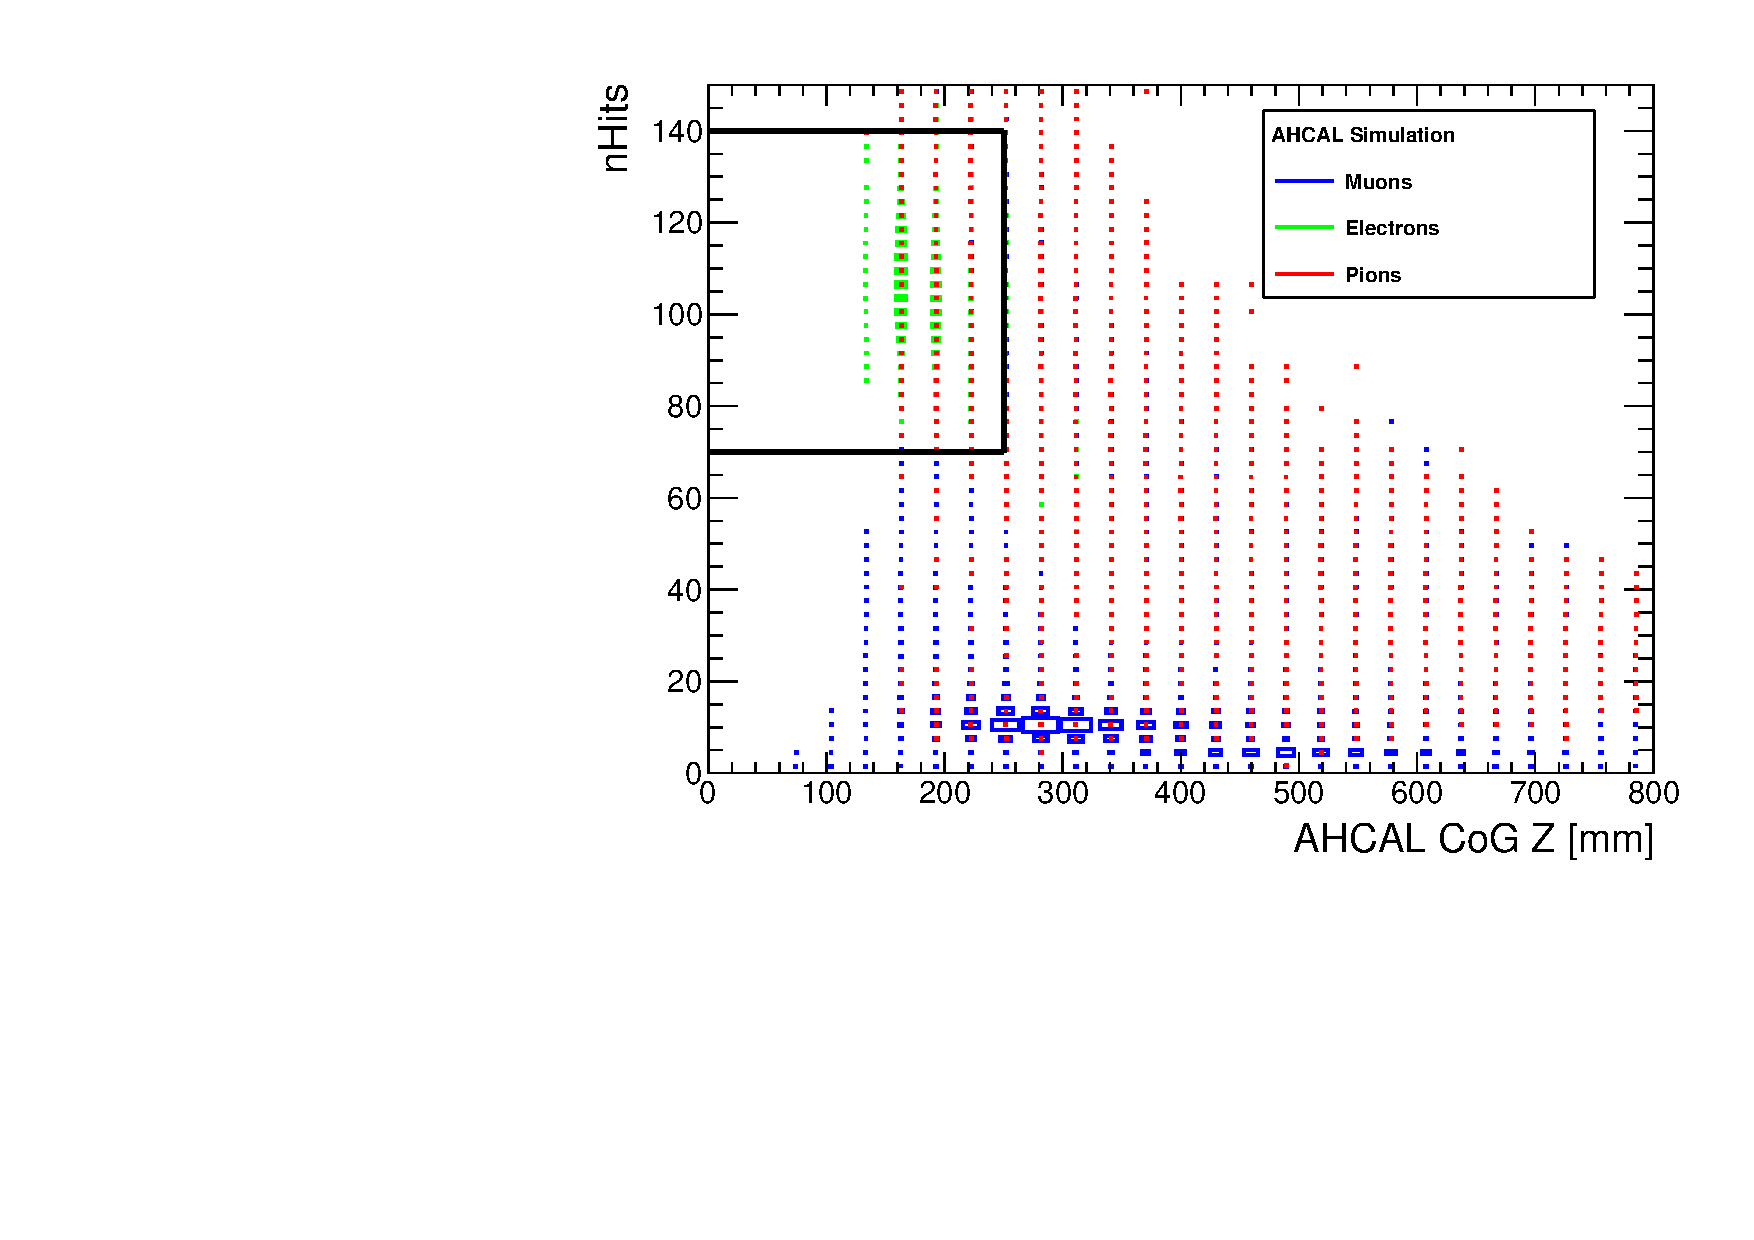
\includegraphics[width=1\linewidth]{../Thesis_Plots/Timing/Electrons/Plots/SelectionCut_nHitsCoGZ_50GeV}
		\caption{50 GeV.} \label{fig:e50GeV_nHitsCoGZ}
	\end{subfigure}
	\hfill
	\begin{subfigure}[t]{0.5\textwidth}
		\centering
		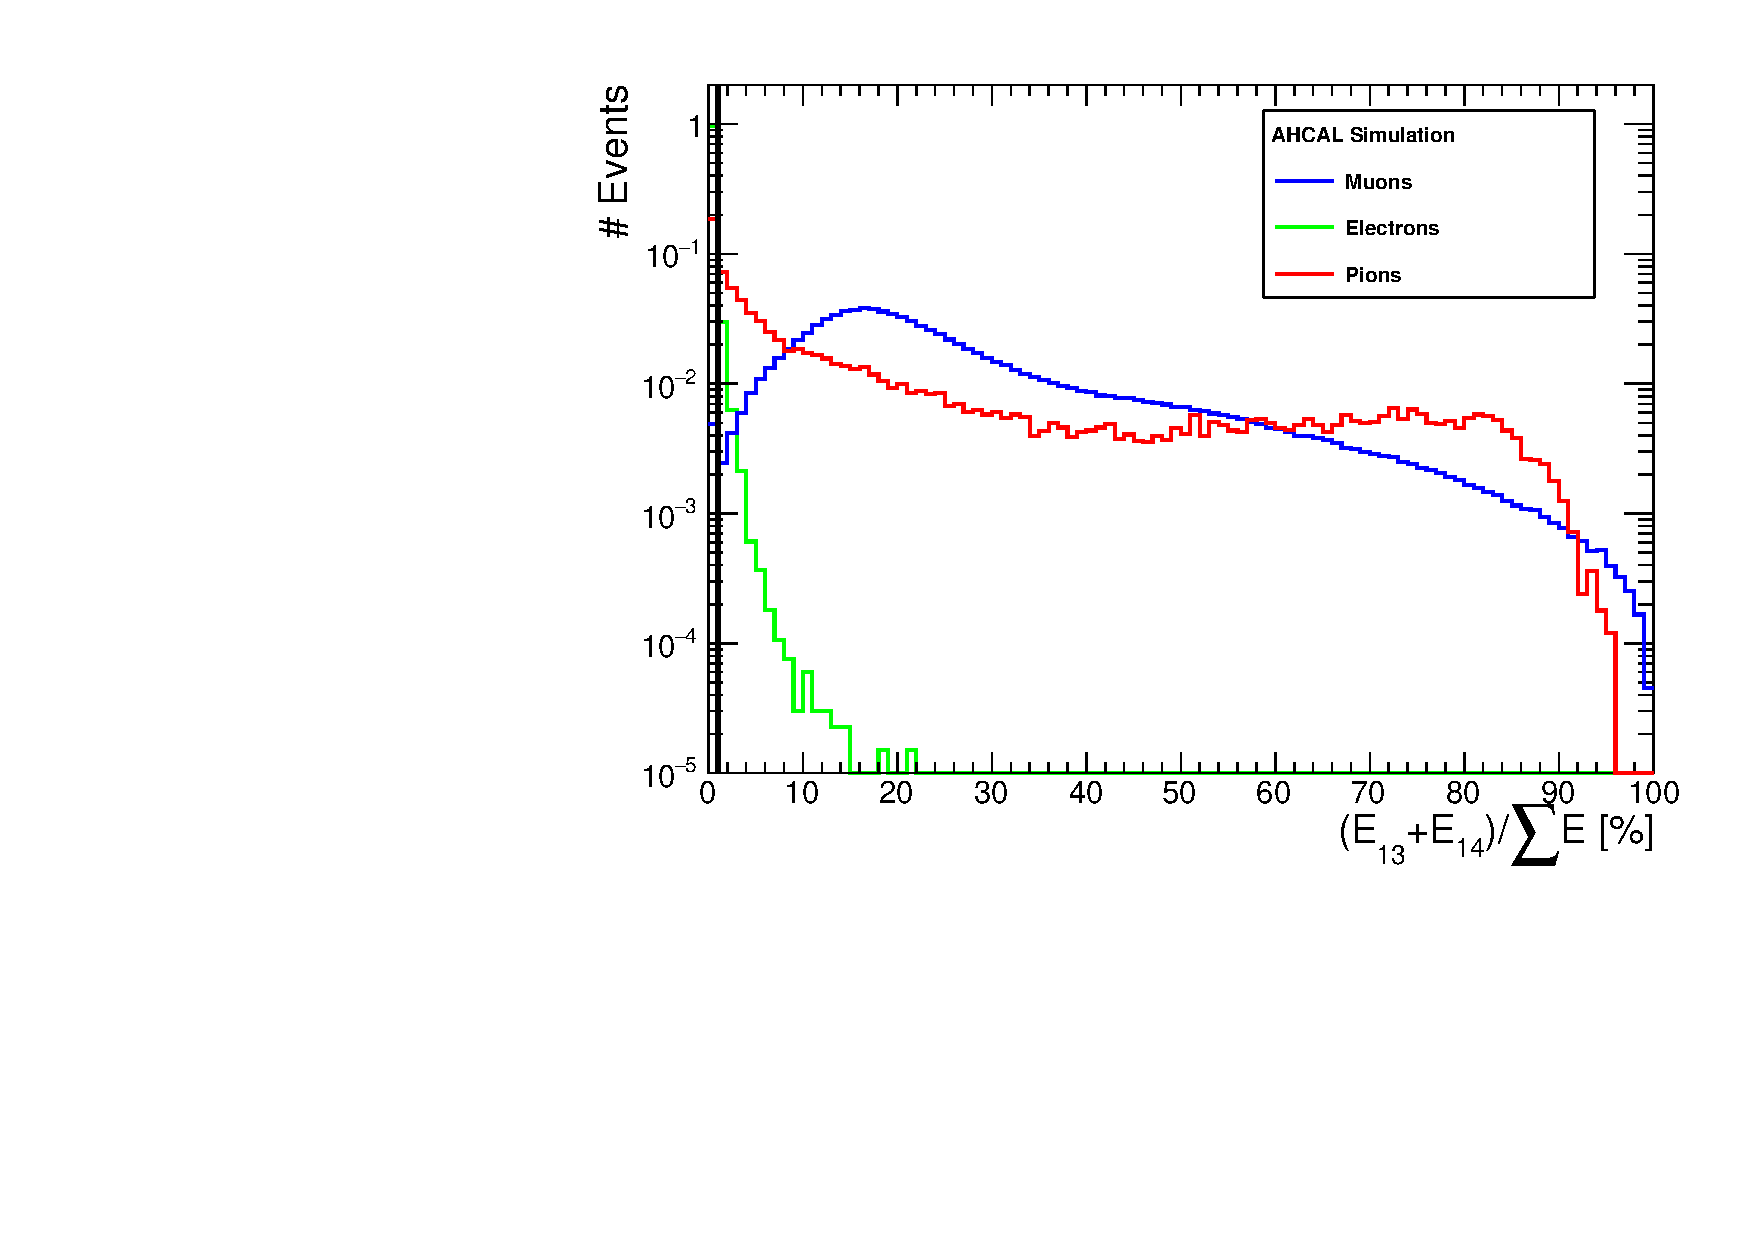
\includegraphics[width=1\linewidth]{../Thesis_Plots/Timing/Electrons/Plots/SelectionCut_EnergyLastLayers_10GeV}
		\caption{10 GeV.} \label{fig:e10GeV_Elast}
	\end{subfigure}
	\hfill
	\begin{subfigure}[t]{0.5\textwidth}
		\centering
		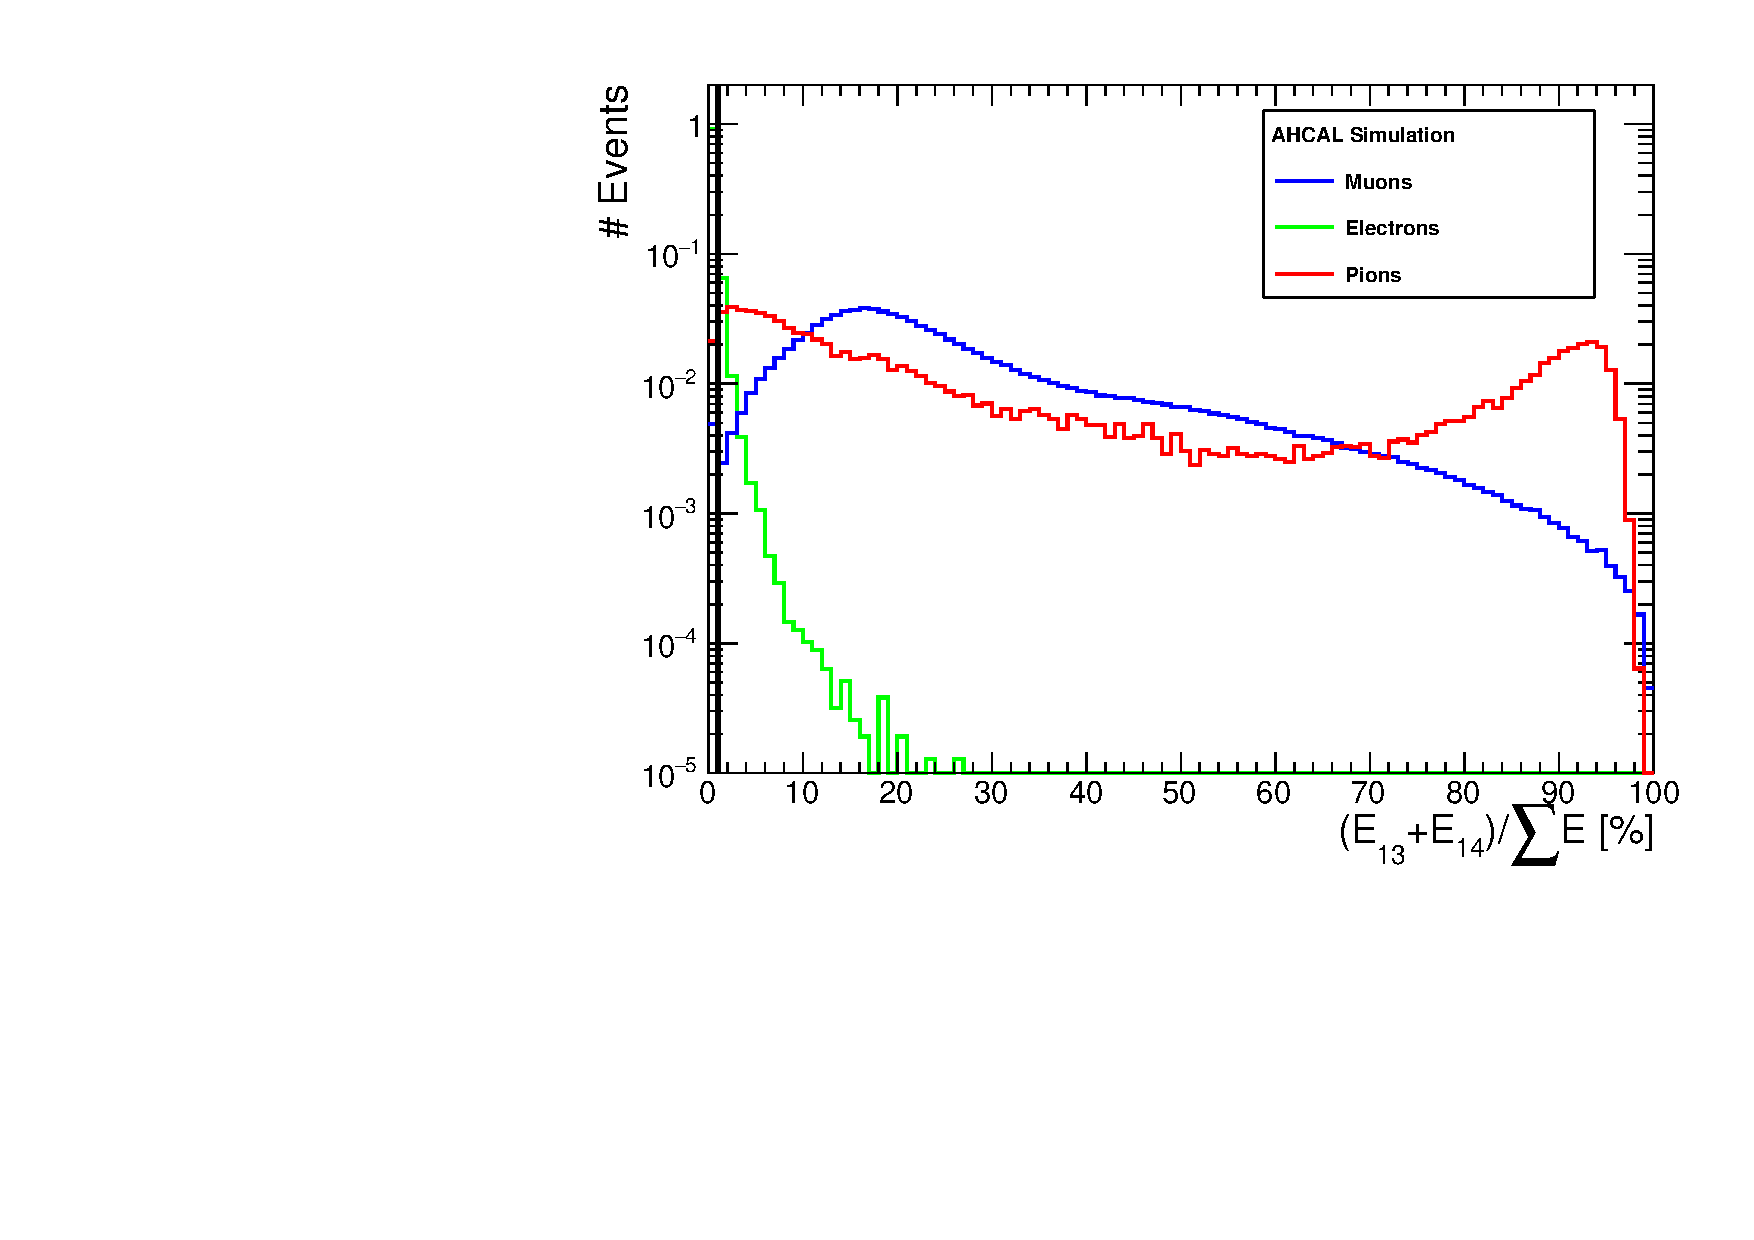
\includegraphics[width=1\linewidth]{../Thesis_Plots/Timing/Electrons/Plots/SelectionCut_EnergyLastLayers_50GeV}
		\caption{50 GeV.} \label{fig:e50GeV_Elast}
	\end{subfigure}
	\caption{Distribution of the variables used in the electron selection of simulated electron and pion beams between 10 and 50 GeV. The muons are simulated at 50 GeV only. These plots were used to determine the best selection criteria for electrons.} \label{fig:electronselection}
\end{figure}

\section{Pion Selection}

A simple selection is performed on pion events. The goal is to reject punch-through pions, muons and possible electron contamination. An \textit{Event Quality} pre-selection is performed utilizing the Cherenkov information, events with no Cherenkov ON are selected. This is only applied to data. The pion selection is based on the same variables: $cog_Z:n_{Hits}$ plane, $(E_{13}+E_{14})/\Sigma E$ and additionally the number of hits in two first AHCAL layers ($N_3+N_4$). The number of hits required per event needs to be over 20 to reject most muons or punch-through pions without cutting on the center of gravity in z in order not to bias the selection on the start of the pion shower. To ensure that the pion showered, the energy in the last two layers of the AHCAL must be over 1\%. And finally, to mitigate possible particle contamination from electrons, the number of hits in the two first AHCAL layer must be under 5. The distributions of each variables used in the selection are shown in figures \ref{fig:pionselection} for simulated 10 GeV and 90 GeV muons, electrons and pions.

\begin{figure}[htbp!]
	\centering
	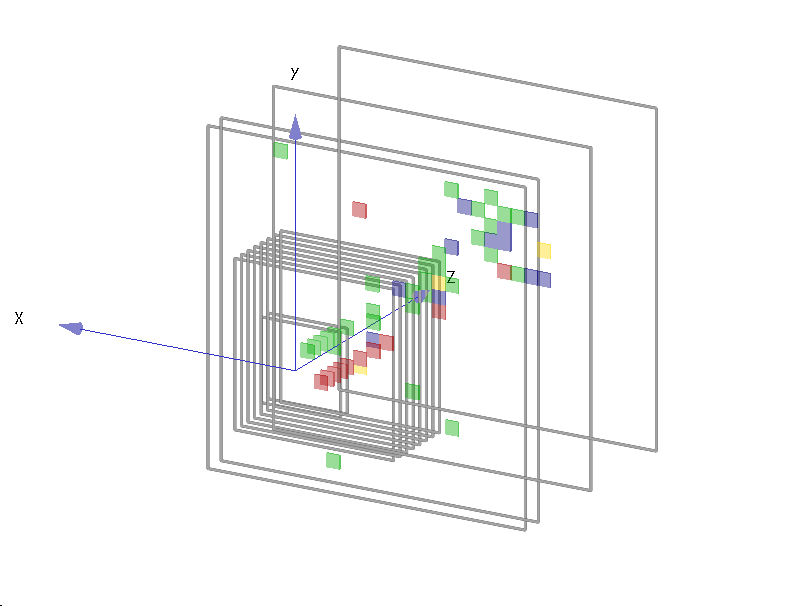
\includegraphics[width=0.7\linewidth]{chap5/fig_AHCAL_timing/Pions/DoubleParticleEventPions.png}
	\caption{Multi-particle event in the 50 GeV pion data sample. The color represents the time of the hit.} \label{fig:DoubleParticleEvent}
\end{figure}

Moreover, after a long investigation, multiple particle events were observed in the data as shown in figure \ref{fig:DoubleParticleEvent}. As no beam instrumentation could be utilized for rejecting these events, a simple rejection method based on time clusters was developed. All hits per event are placed and ordered in time in a vector. For each hits after 50 ns, a window of 30 ns is looked after and the number of hits in that window is counted. If the number of hits is over 5, it is counted as a late cluster. The event is rejected if the number of late clusters is over zero. This method works because if an event has several particles, the time reference of the event is generated by the first particle, then in this case, the second particle will have all the hits late relative to the time reference and thus the event will be rejected with this method. The method was based on data in order to remove efficiently multi-particle events. The multi particle event rejection has been checked on simulated data and affects the selection between <0.1\% up to 2\% from 10 to 90 GeV pions.
These multi-particle events are greatly suppressed in data using this method but due to the calorimeter not being fully equipped, some contamination may remain in the data.

A detailed description of the selection cuts are shown in table \ref{table:pion_sel}.

\begin{table}[htb!]
	\centering
	\caption{Efficiency of the pion selection for beam energies between 10 and 90 GeV.}
	\label{table:eff_electron}
	\begin{tabular}{@{} llll @{}}
		\hline
		\textbf{Beam Energy} & \textbf{$\epsilon_{\mu}$} & \textbf{$\epsilon_{e}$} & \textbf{$\epsilon_{\pi}$}\\
		\hline
		10 GeV & <0.1\% & <0.1\% & 29.9\%\\
		30 GeV & 0.9\% & <0.1\% & 50.3\%\\
		50 GeV & 0.9\% & <0.1\% & 51.1\%\\
		70 GeV & 0.9\% & <0.1\% & 51\%\\
		90 GeV & 0.9\% & <0.1\% & 50.2\%\\
		\hline
	\end{tabular}
\end{table}

\begin{figure}[htbp!]
	\begin{subfigure}[t]{0.5\textwidth}
		\centering
		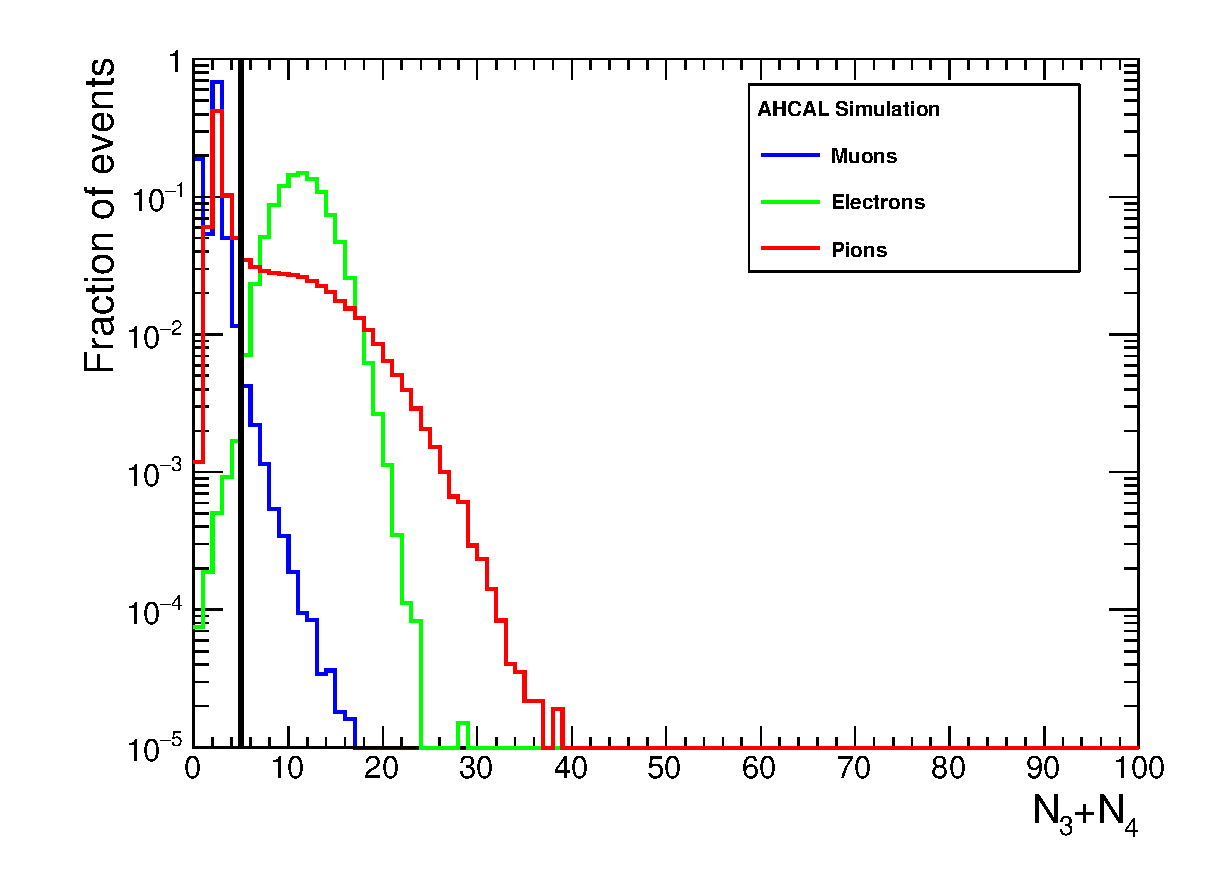
\includegraphics[width=1\linewidth]{../Thesis_Plots/Timing/Pions/Plots/SelectionCut_N3N4_10GeV}
		\caption{10 GeV.} \label{fig:pi10GeV_N3N4}
	\end{subfigure}
	\hfill
	\begin{subfigure}[t]{0.5\textwidth}
		\centering
		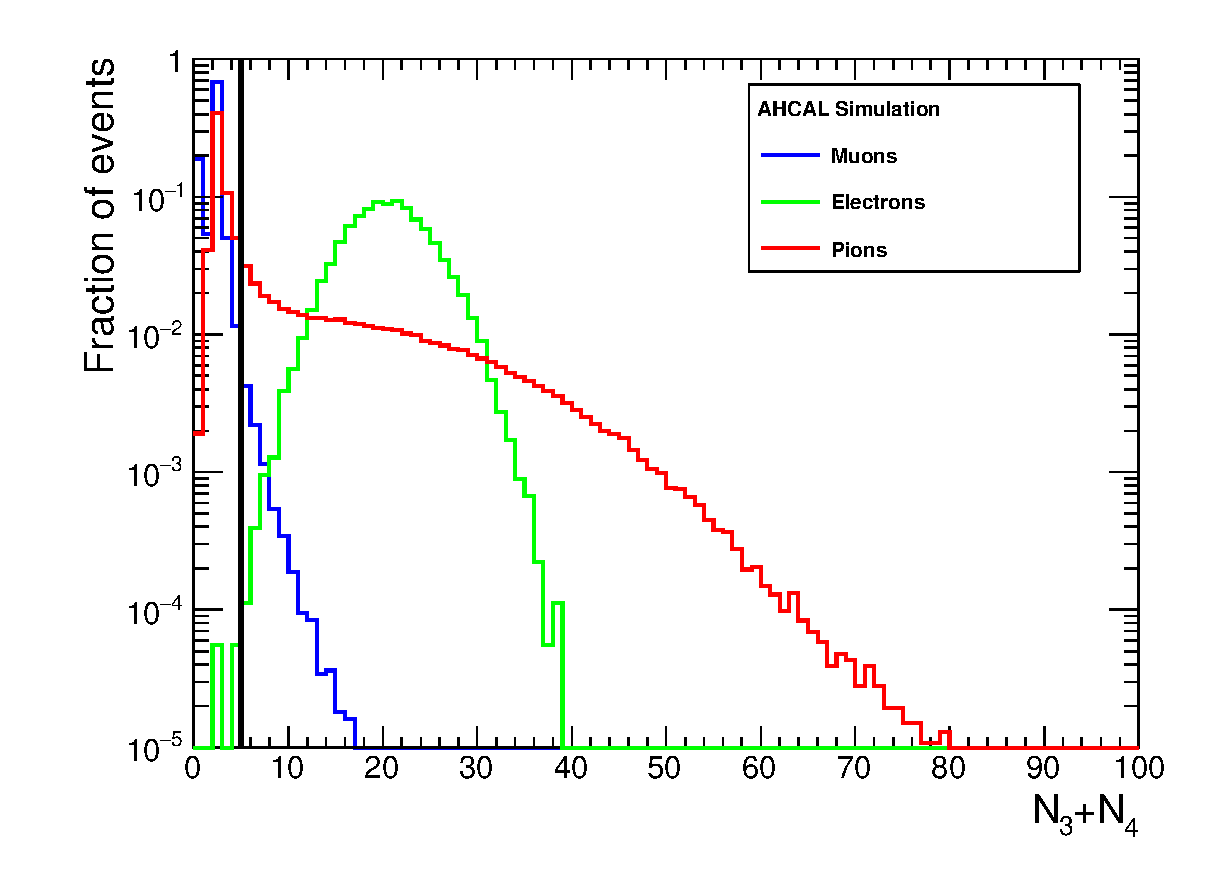
\includegraphics[width=1\linewidth]{../Thesis_Plots/Timing/Pions/Plots/SelectionCut_N3N4_90GeV}
		\caption{90 GeV.} \label{fig:pi90GeV_N3N4}
	\end{subfigure}
	\hfill
	\begin{subfigure}[t]{0.5\textwidth}
		\centering
		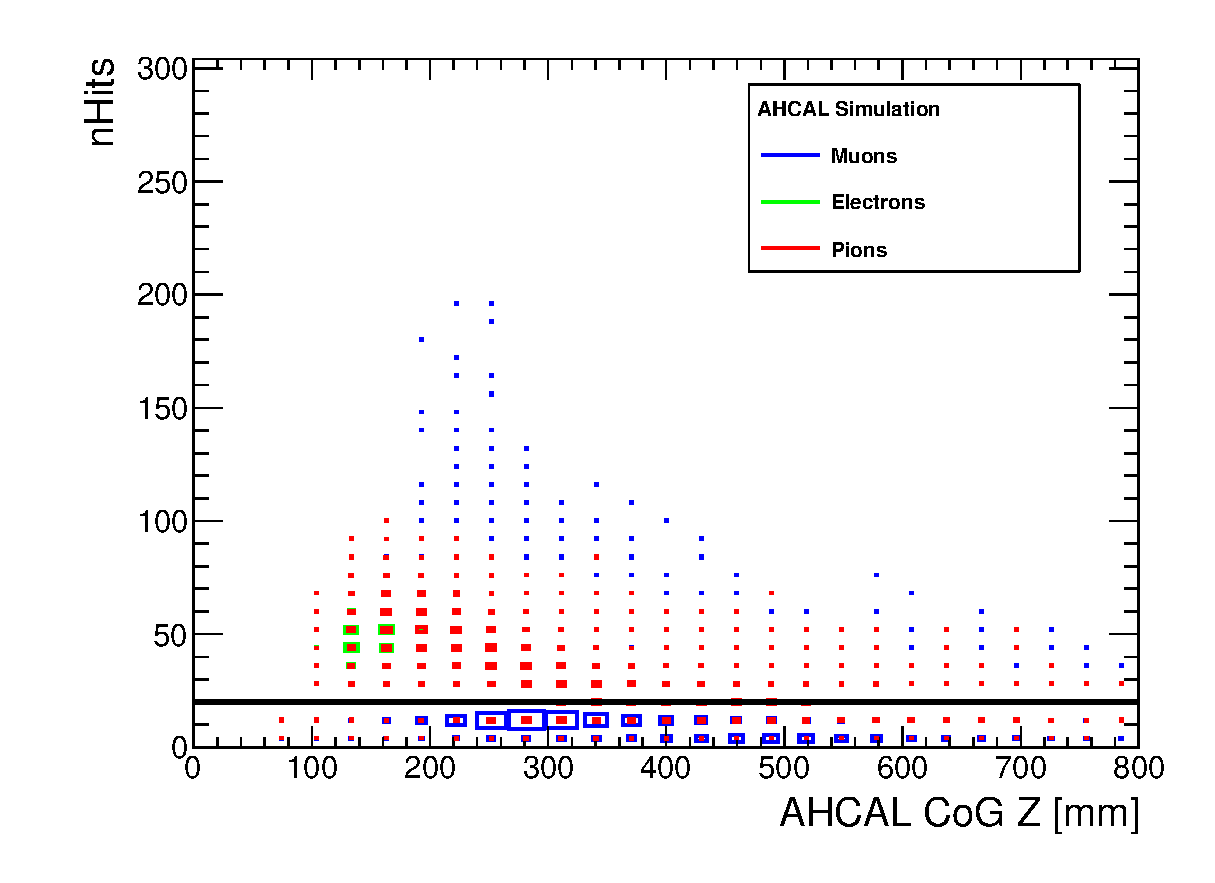
\includegraphics[width=1\linewidth]{../Thesis_Plots/Timing/Pions/Plots/SelectionCut_nHitsCoGZ_10GeV}
		\caption{10 GeV.} \label{fig:pi10GeV_nHitsCoGZ}
	\end{subfigure}
	\hfill
	\begin{subfigure}[t]{0.5\textwidth}
		\centering
		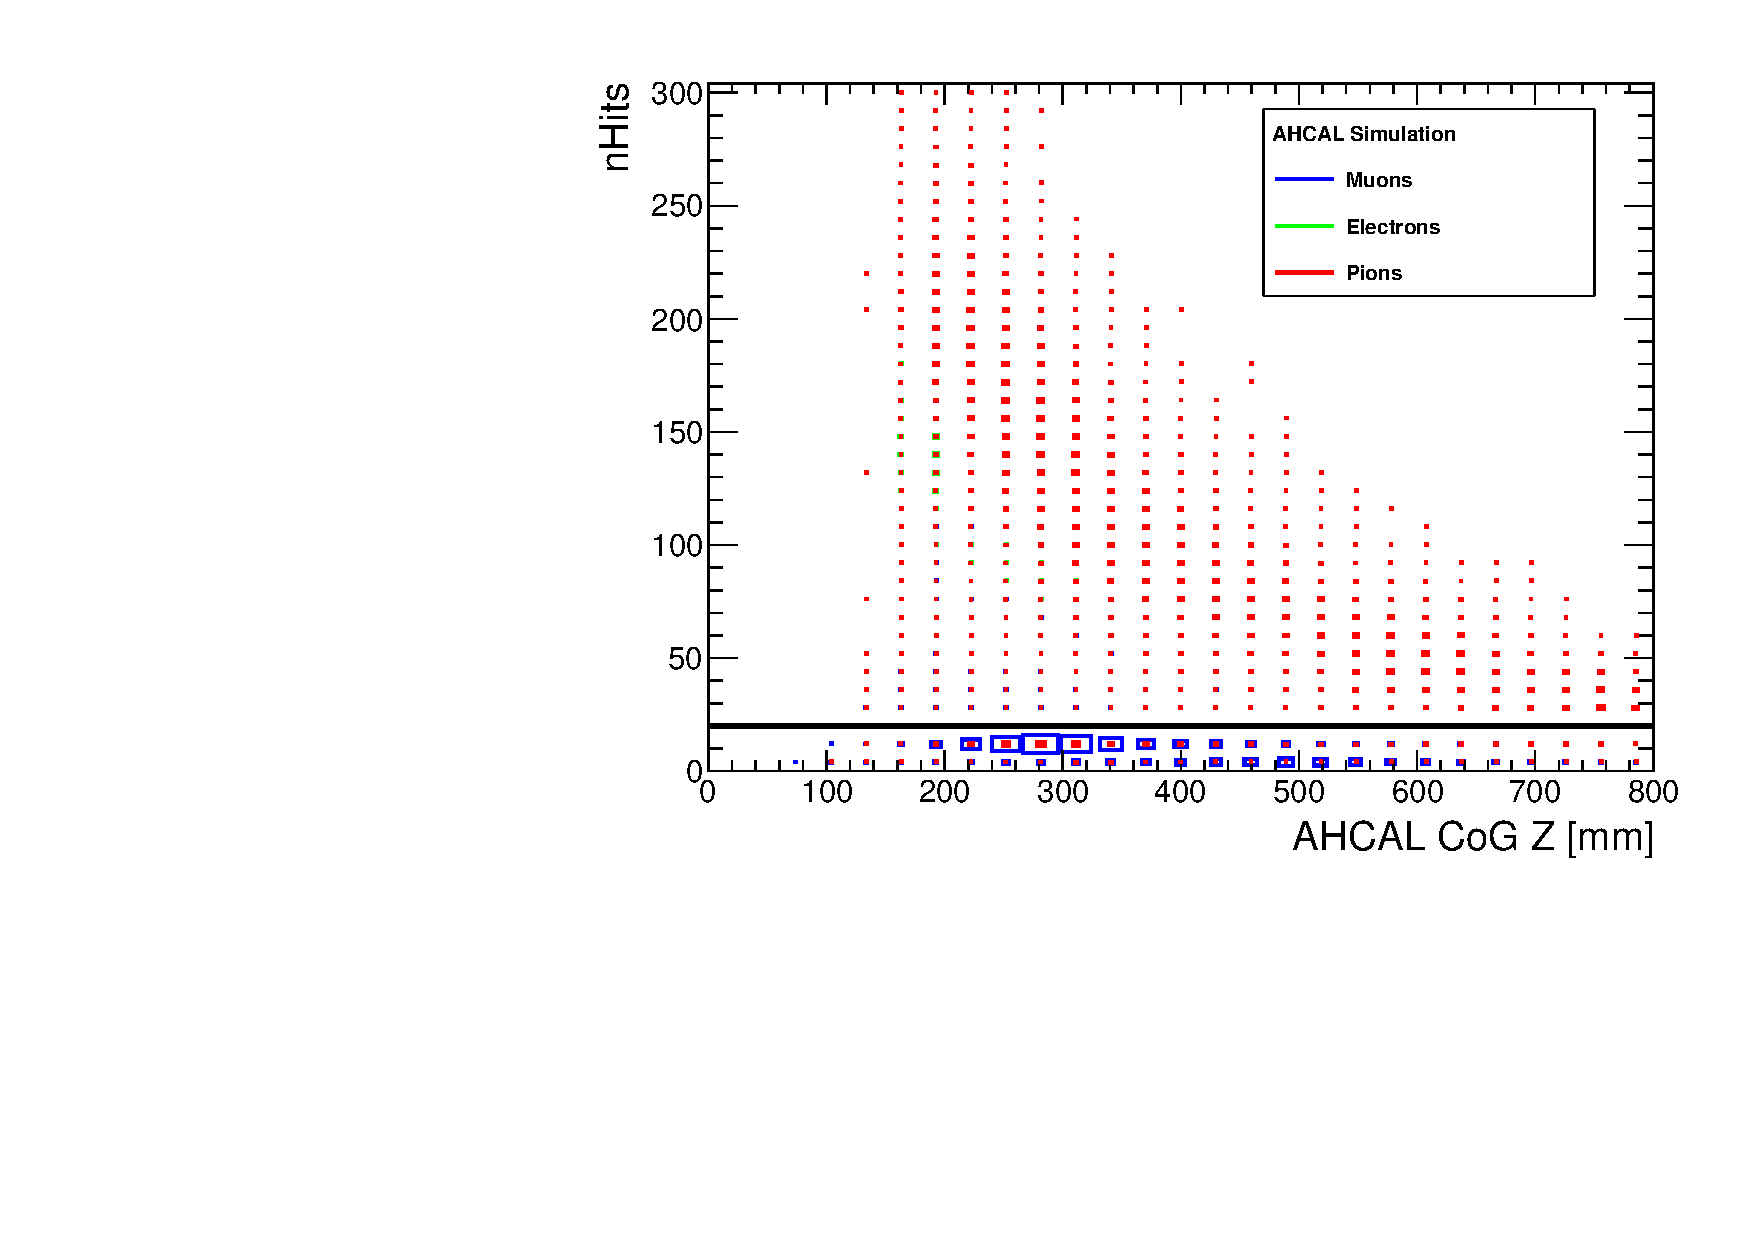
\includegraphics[width=1\linewidth]{../Thesis_Plots/Timing/Pions/Plots/SelectionCut_nHitsCoGZ_90GeV}
		\caption{90 GeV.} \label{fig:pi90GeV_nHitsCoGZ}
	\end{subfigure}
	\hfill
	\begin{subfigure}[t]{0.5\textwidth}
		\centering
		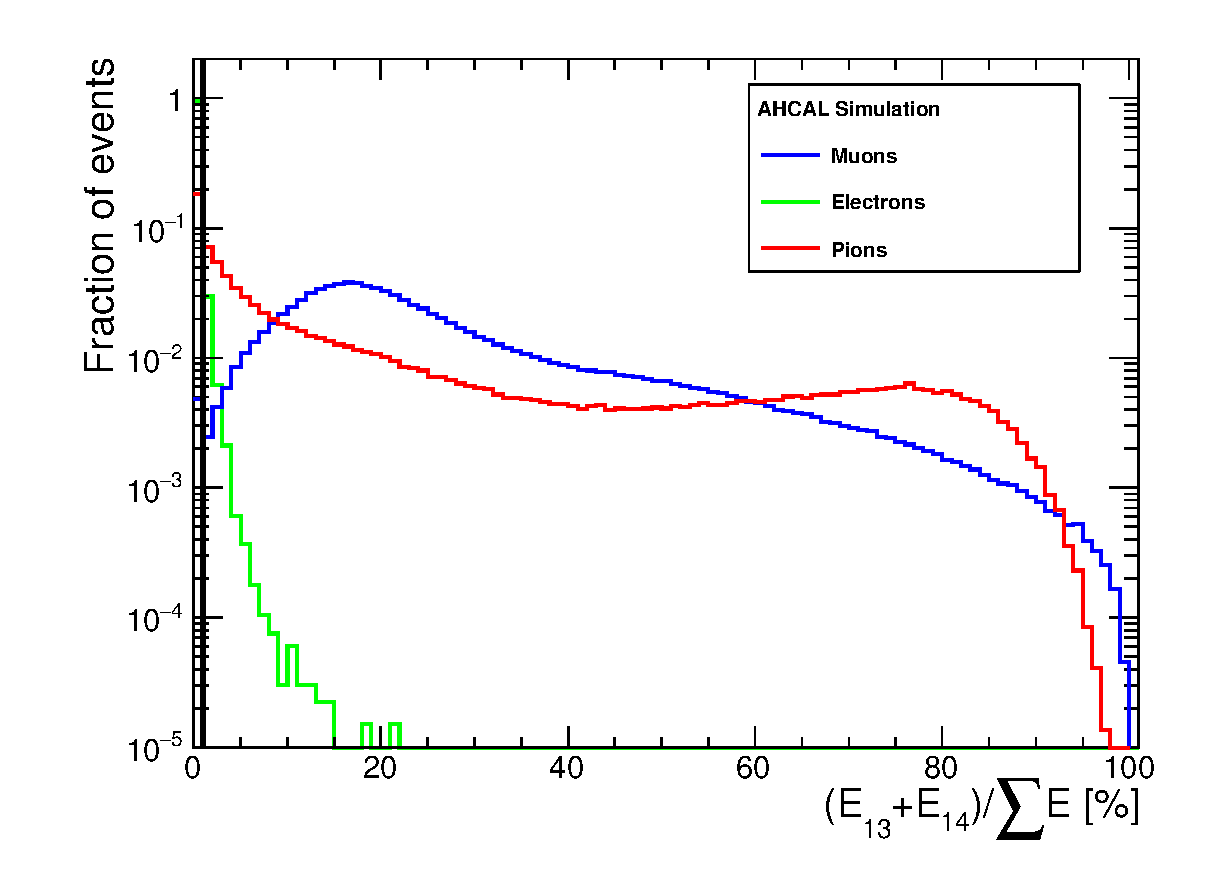
\includegraphics[width=1\linewidth]{../Thesis_Plots/Timing/Pions/Plots/SelectionCut_EnergyLastLayers_10GeV}
		\caption{10 GeV.} \label{fig:pi10GeV_Elast}
	\end{subfigure}
	\hfill
	\begin{subfigure}[t]{0.5\textwidth}
		\centering
		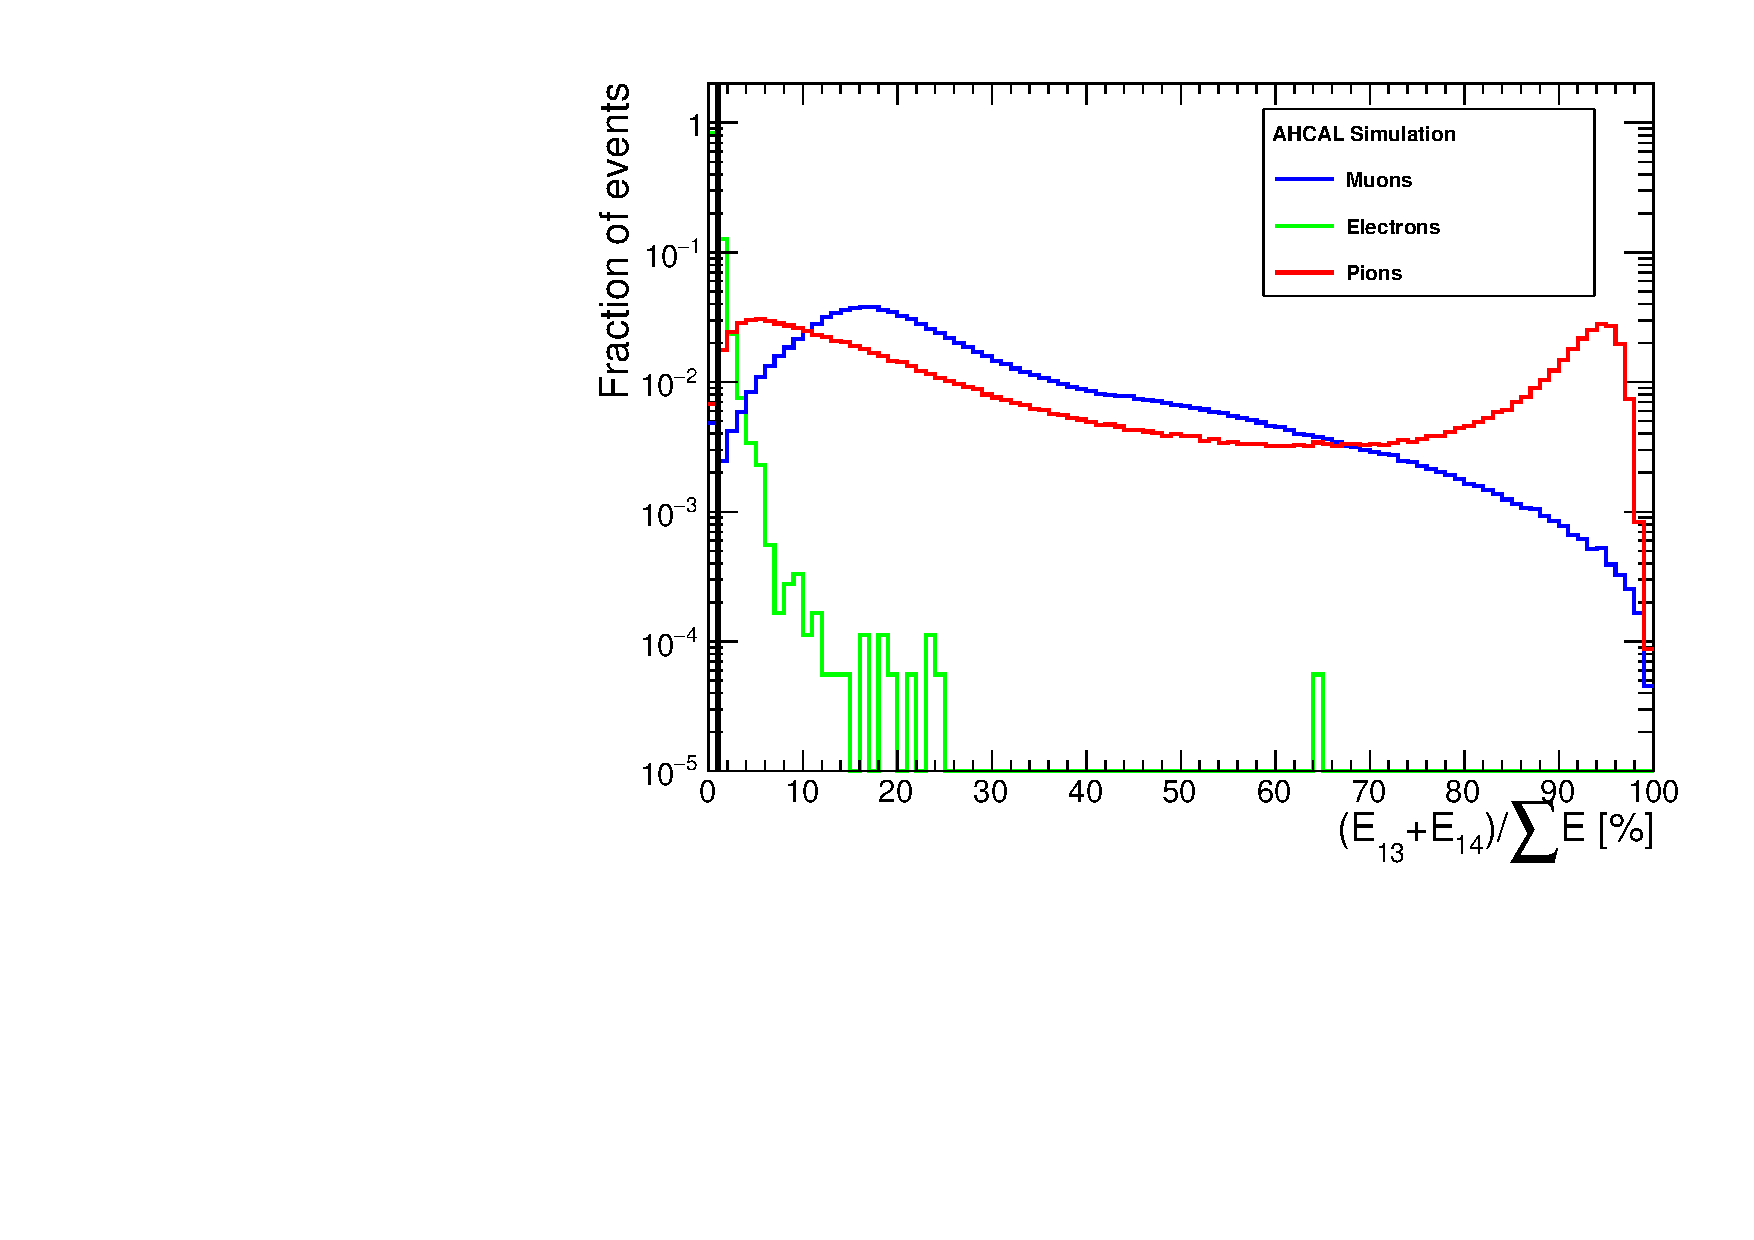
\includegraphics[width=1\linewidth]{../Thesis_Plots/Timing/Pions/Plots/SelectionCut_EnergyLastLayers_90GeV}
		\caption{90 GeV.} \label{fig:pi90GeV_Elast}
	\end{subfigure}
	\caption{Plots of simulated muon, electron and pion beams between 10 and 90 GeV. Theses plots were used to determine the best selection criterium for pions.} \label{fig:pionselection}
\end{figure}

In appendix \ref{appendix:SimulationVal}, more distributions are available to show the agreement between data and simulations for muons, electrons and pions.

\section{Chip rejection}

For each type of data analyzed, a careful check of each chip has been performed. For all the data collected, the layer 11 is rejected. For the muon data, only a single chip (157) shows a strange behavior likely because the IDACs on this chip were broken.

For the electron data, a relative fraction of hits $r$ following the equation \ref{eq:fraction_rejection} was looked at. If this fraction $r$ is below 98\%, the chip is rejected. This means that most of the hits in the event are in the core of the distribution between -50 and 50 ns. With this method, 20 chips are rejected.
\begin{equation} \label{eq:fraction_rejection}
	r = \frac{1}{N} \left|\int_{50 ns}^{200 ns} \frac{dN(t)}{dt} dt - \int_{-200 ns}^{50 ns} \frac{dN(t)}{dt} dt\right|
\end{equation}
For the pion data, applying the same method as for electrons is not possible due to the late tail related to delayed energy deposition from neutrons. The same chips as for electrons were rejected but additionally, each chip time distribution after correction were manually checked and chips presenting an abnormal shape were discarded. This way additionally 16 chips are rejected. This leaves 44 chips in the pion analysis. A detailed table of the rejected chips can be seen in appendix \ref{appendix:rejection}.

\begin{figure}[htbp!]
	\begin{subfigure}[t]{0.5\textwidth}
		\centering
		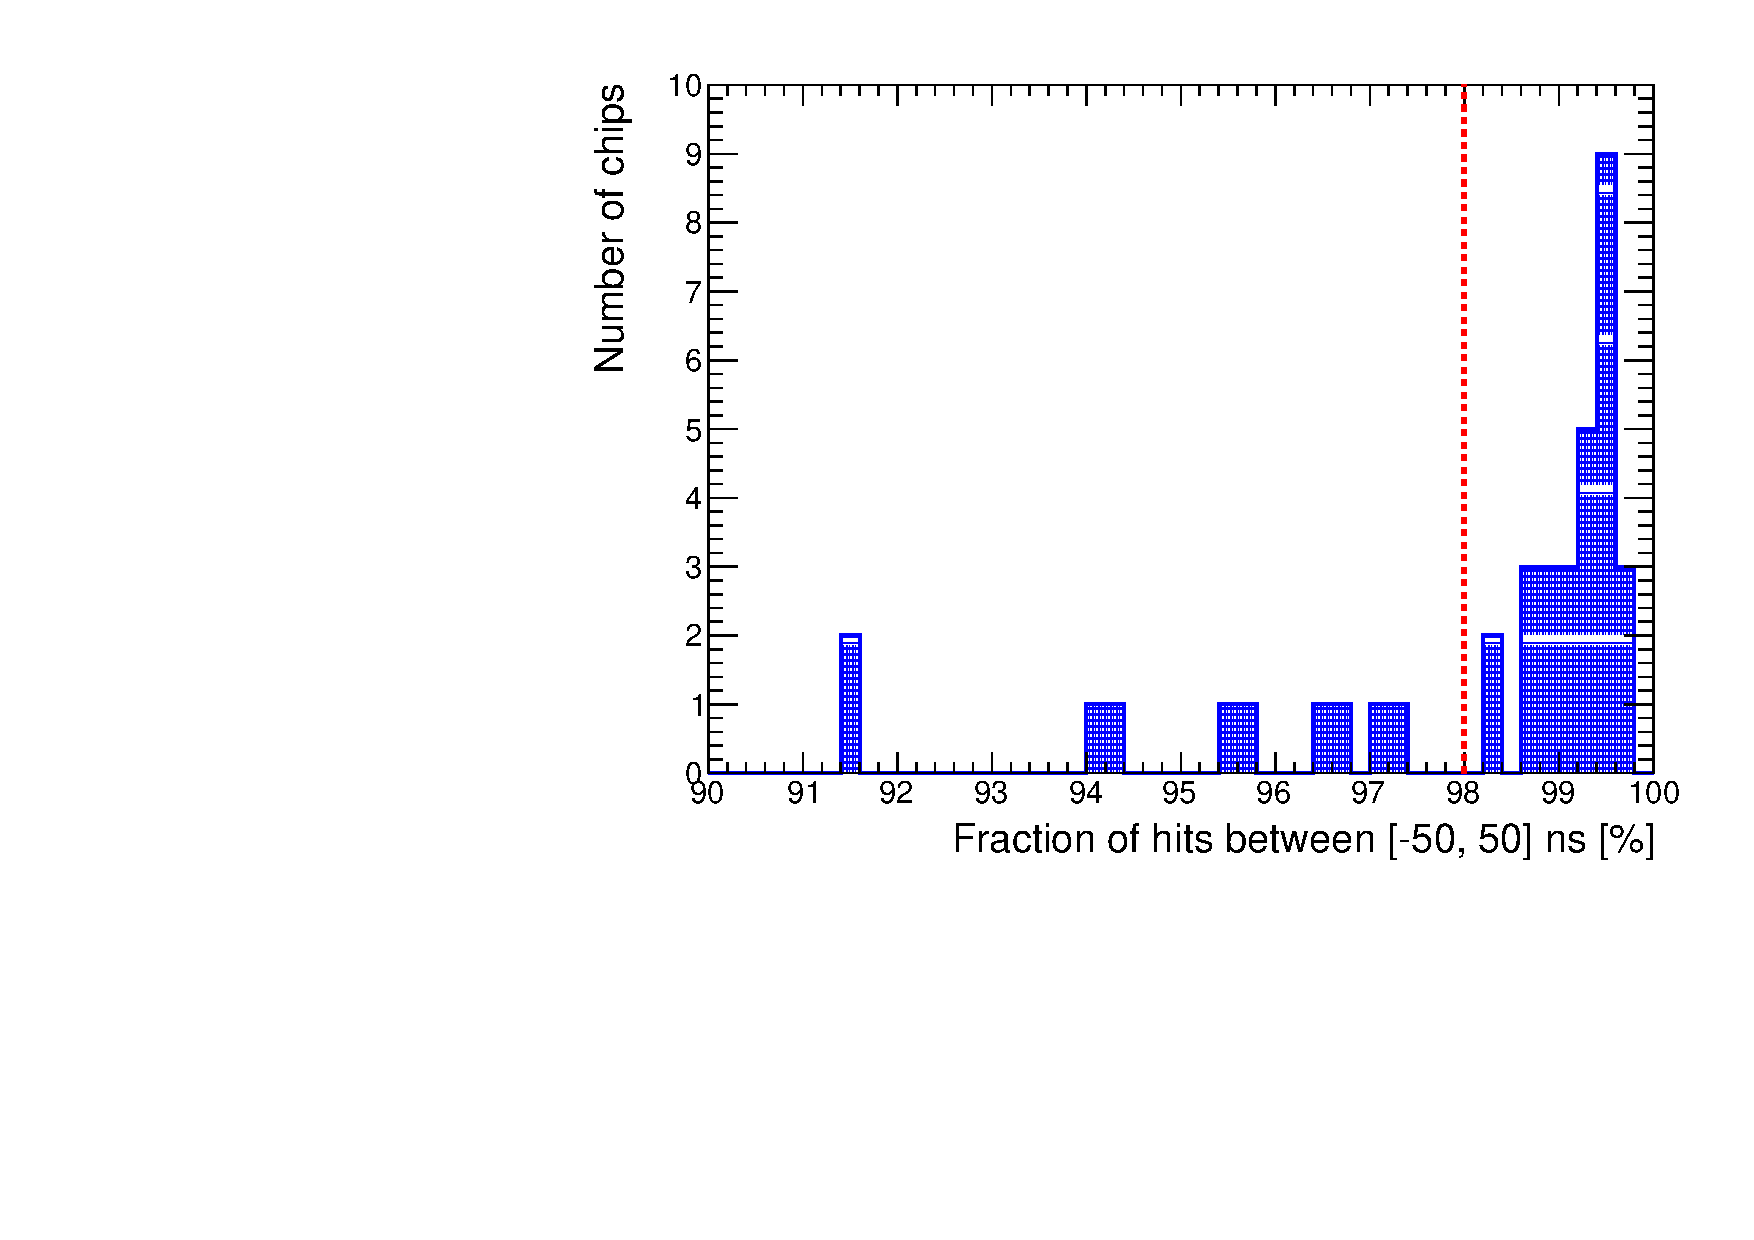
\includegraphics[width=1\linewidth]{../Thesis_Plots/Timing/Electrons/Plots/FractionRejectedChips.pdf}
		\caption{.} \label{fig:FracRejChip}
	\end{subfigure}
	\hfill
	\begin{subfigure}[t]{0.5\textwidth}
		\centering
		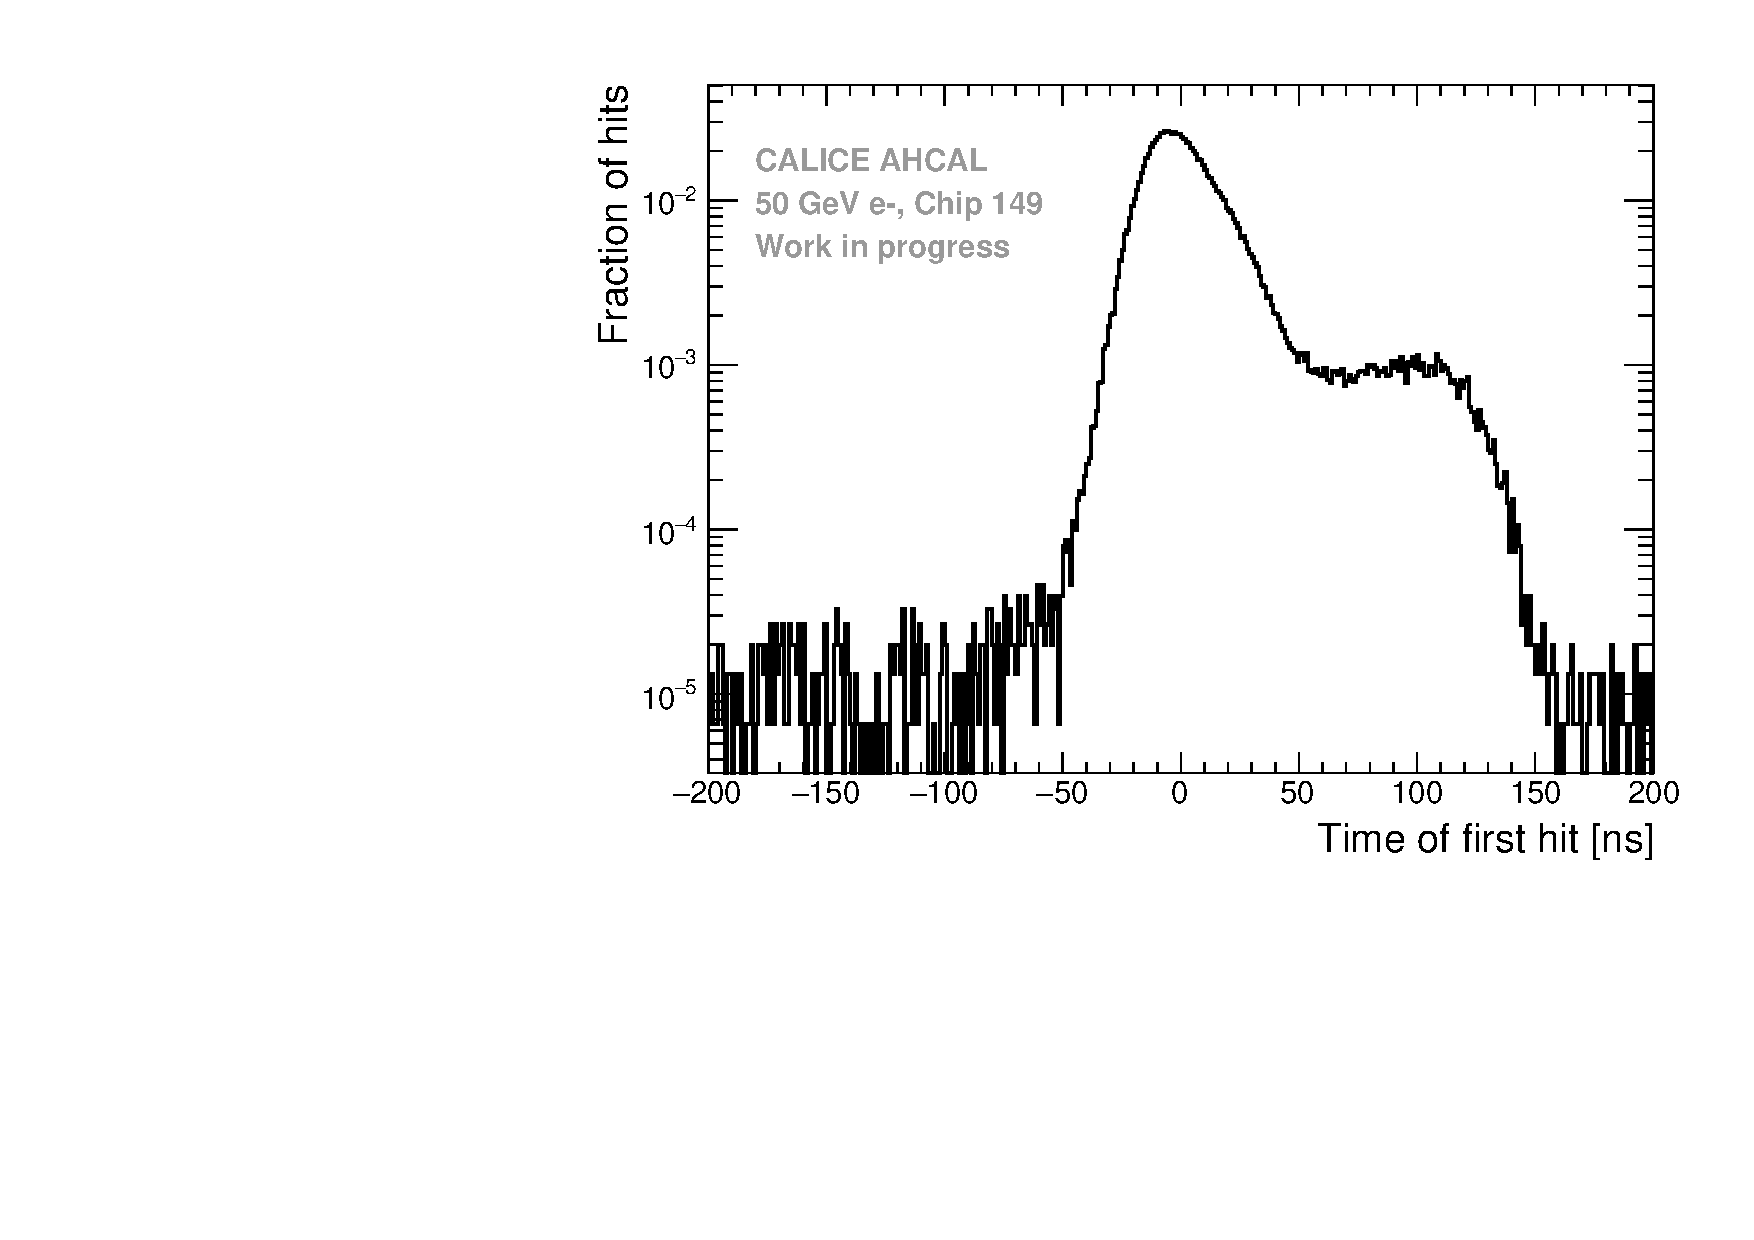
\includegraphics[width=1\linewidth]{../Thesis_Plots/Timing/Electrons/Plots/ExampleBadChip149.pdf}
		\caption{.} \label{fig:ExBadChip}
	\end{subfigure}
	\caption{\subref{fig:FracRejChip}) Distribution of the fraction of hits between -50 and 50 ns for 50 GeV electrons. Each entry corresponds to a chip. The red line represent the cut applied to reject bad chips. \subref{fig:ExBadChip}) Example of a bad chip that is rejected with this method (Chip 149).}
\end{figure}
